\chapter{Conclusion: Paradigms and Possibilities}
%outline where the diss has been to set up some framing
The chapters of this dissertation build on one another to create what seems to be an isolated, self-supporting data pipeline in which terms like jazz, harmony, chord, progression, and syntactic function receive narrowly specific (and idiosyncratic) definitions.  Building a corpus of jazz performance in MIDI format, tallying tiny-duration, locally-transposed scale degree sets as chords, and clustering those chords based on the statistics of their temporal deployment produce jazz harmonic claims connecting analytical abstraction to performance data through a complex -- but specific and frameable -- series of computational procedures.  It is clear that (or how) these claims are supportable within the ontological framing given here; less clear is their status with regard to traditional theories of jazz (and non-jazz) harmony.  The preceding three chapters look quite different from traditional harmonic theory discourse, and the semiotic framing of Chapters 2 and 4 implies that the resulting claims might not ``prove" or ``disprove" traditional harmonic theoretical claims directly.  Instead, the pipeline might produce similar-seeming analytical interpretants functioning as analytical homophones; they \emph{sound} like harmonic theory, but the two may rely on incommensurate epistemologies.

What I advocate here, in its most generally Kuhnian sense, is a kind of paradigm shift, or at least the simultaneous adoption of a new paradigm\footnote{Cite Kuhn, \emph{Structure of Scientific Revolutions}.}  Extant successful jazz harmonic theories employ a particular epistemic framework (or, more properly, a closely-related set of frameworks), a language in which to write claims, as I will discuss below.  At the ground level, these frameworks involve ways of defining the terms of the discourse, like ``chord" and ``progression," as well as the accepted data to which the claims of the discourse should be accountable, like ``lead sheets" or ``score transcriptions."  But any functional paradigm also consists of an agreed-upon set of production rules for claims, a series of methods or processes used to generate statements about the data in a discursively-stable way.  Put reductively, I consider a paradigm to consist of discursively-useful statements, a domain deemed relevant and appropriate for investigation, and methods which the community operating under the paradigm considers sufficient for furnishing a proof of or offering support for the discursive statements.

Theorists in any field may (and do) differ regarding which claims are ``true" under the paradigm, and this is the source of most productive academic discourse.  But when the claims written in a paradigmatic language become sufficiently complex, new paradigms may be proposed; as Kuhn notes, new paradigms typically gain supporters in the field by re-writing claims accepted under the old paradigm in terms of the new.  If the proponents of the new paradigm can demonstrate that the same (\emph{a priori} useful) claims are reachable in a new way, and if they can argue that the new paradigm provides a framework more flexible, generalizable, justifiable, or elegant, then segments of the discourse may migrate, choosing to identify problems, perform research, and present their results in terms of the new paradigm.  A paradigm shift may undermine few or none of the claims made in the old paradigm, replacing instead the assumptions underlying and language describing the claims.

Seen on this basis, any new paradigm confronts three types of inquiry:
\begin{enumerate}
	\item \textbf{Reproduced claims}: Much of the heavy-lifting of this dissertation results in reproducing old knowledge in new terms.  When chapters 3 and 4 produce clustered categories of phonetic and syntactic similarity, the results partly subsume  traditional expectations regarding tertian-stack, root-based, hand-analyzed category assignment.  Work of this kind reproduces statements like ``$I$ triads behave like $vi$ triads," but it does so by a completely different set of processes accountable to different data.
	\item \textbf{Unreproduced claims}: Some types of claim produced by other paradigms cannot be rewritten (either simply or at all) in terms of the framework established in the preceding chapters.  Some of these unreproduced claims demonstrate weaknesses in the new paradigm, places where it fails or requires supplementation.  Others might indicate failures of extant paradigms, claims which might fail to be reproduced because they are only consistent or relevant in the context of their particular frameworks.  Interpreting the status of unreproduced claims with regard to existing and new paradigms involves complex considerations of framing and discursive utility.
	\item \textbf{New claims}: The data-driven framework which allows the reproduction of many pre-existing claims also broadens the class of claims possible.  By stripping away assumptions about chord structure, root, and successive immediacy, constructing and examining temporal progression regimes affords statements ill-formed under other paradigms, including statistically-supportable claims about the behavior of chords at a distance and similarity measures between chords with arbitrarily different pitch structures.
\end{enumerate}
The first and third kinds of inquiry enumerated above represent a straight-forward argument for a paradigm shift in discourse on jazz harmony.  The second kind functions to destabilize the totalizing nature of that shift, pointing to the limits of the new paradigm and identifying places where other paradigms provide better, more nuanced, and more useful claims.  The examination of unreproduced claims encourages the suspension of judgment regarding which conceptual proof structures are valid in favor of imagining which kinds of discourse might accomplish worthy goals.

Chapters 2-4 largely constitute demonstrations of claim reproduction.  Chapter 2 extracts voicings and scale-degree sets (two particular interpretants based on indices standing for ``chords") in line with the theoretical expectations of Mehegan, Martin, and Levine.  Chapter 3 translates notions of chord behavior into explicitly temporal syntactic terms, reproducing the most basic harmonic expectation found in elementary jazz harmonic discourse (like $ii - V - I$) from progression statistics in three temporal regimes.  With syntactic temporality as a ground, Chapter 4 reproduces chord categorization and substitution schemes common to a variety of jazz manuals with a different proof structure.  If these kinds of claims have discursive utility, attending to temporal progression regimes clearly affords their reproduction, albeit from a different domain -- a highly individualized corpus of unquantized MIDI performance, rather than notational transcriptions of tunes or recordings -- and with a different idea of what furnishes proof -- statistics produced without hand-annotation.

In what follows, I will compare this work to the work of other jazz theorists, paying particular attention to existing claims unreproduced under my temporal syntactic paradigm.  I will then suggest new directions afforded by the computational semiotic framing of Chapters 2-4.  At the end of the chapter, I will also suggest (somewhat paradoxically) that the very nature of a data-driven, corpus-based paradigm might amplify the impact of destabilizing, unreproduced claims, rendering the heterogeneous remainders left behind by dominant paradigms more legible and accessible.  Data-driven harmonic analysis might be seen to provide tools capable of both making powerful generalizations and undermining their hegemonic influence.

\section{Unreproduced Claims: Comparing frameworks}
%But how do we pull apart the structure of the old paradigm, theoretically?  Close reading of Strunk, Waters, and Terefenko.
%Pull in Wollheim's types of formalism

While claims regarding the typical deployment of chords with respect to their local key centers can be well-captured by temporal clustering, several related types of harmonic claim find no ready translation.  Two traditional discursive methods -- that of discussing harmonic prolongations, and that of performing close score analysis of functional harmony -- do not exhaust the space of unreproduced claims, but they may capture the most important omissions.  Understanding the nature and framing of unreproduced claims from these paradigms requires an examination of more than the intuitive usefulness of the claims themselves.

Both theoretical processes partake of what might be called \emph{formalism} in particular ways, abstracting harmonic claims from the musical surface meant to capture information about performance independent of a variety of other contextual factors and features.  These abstractions, reductions, and partitions of features are not entirely unique to the musical domain, and in discussing them, I will make reference to the descriptions of analogous formalism in the theory and history of art offered by Richard Wollheim.\footnote{Cite Wollheim, especially \emph{Formalism and Its Types}, and to a lesser extent \emph{Art and Its Objects}.}  Following the mid-century backlash of syntactic and symbolic formalists against early twentieth-century biographical intentionalism,\footnote{By this, I mean the wave of formalist projects in the 1950s and 1960s which share George Kubler's eloquent description of art praxis as a dark mine; for Kubler, investigating the personal histories of the individual artists-\emph{cum}-miners precludes an appropriate focus on the (formalist) nature of the composition and topography of the material available for mining.  Kubler's work presents a complex historical formalism, and his abstraction of stylistic change in terms of mathematically-inspired chains of replication is ultimately brought into contact with Wollheim's formalist critiques in the work of Whitney Davis.  See Kubler, \emph{The Shape of Time}, and Davis, \emph{Queer Beauty} and especially \emph{A General Theory of Visual Culture}.}  Wollheim offers a series of corrective critiques regarding the formalist (over)reaction.  Concerned with art-historical claims regarding the ``essence" of particular works of art as being fully separable from and analyzable without representational or historical information, Wollheim offers in \emph{Formalism and Its Types} an analytic typology of formalisms, each type of which warrants specific structural objections.

In what follows, I bring Wollheim's notion of manifest formalism to bear on the jazz prolongational work of Steven Strunk and its response and elaboration in the work of Keith Waters.  Waters's nuanced position will lead to a discussion of latent formalism in jazz harmonic analysis, and I will follow Wollheim's description of particularly syntactic latent formalism to situate my harmonic claims with regard to close readings and pedagogical techniques offered by Darius Terefenko.\footnote{The latent formalism of Wollheim's critique is a significant influence on Whitney Davis's use of the term, which I invoked in Chapter 1.}

\subsection{Prolongation as Manifest Formalism}
%Strunk jazz prolongation, Waters's response, translation into Wollheim
%manifest formalism as drive-by attack on Schenker, pivot toward latent formalism

%Strunk
The Spring 2016 issue of \emph{Music Theory Spectrum} offers an unusual chance to compare very similar jazz harmonic analyses from two different scholars which differ primarily in their justification schemes.  Published adjacent to one another, Steve Strunk's ``Tonal and Transformational Approaches to Chick Corea's Compositions of the 1960s" and Keith Waters's response, ``Chick Corea and Postbop Harmony," both engage with the harmonic language of Corea's ``Windows" (1966).\footnote{Cite Strunk and Waters.}  The published lead sheet for the tune is reproduced here as Figure~\ref{windows}.  In an attempt to explain the ``tonal and harmonic ambiguity" of ``Windows," Strunk provides Schenkerian voice-leading graphs and layered harmonic reductions based on Corea's published lead sheet for the tune.  The two analytical possibilities Strunk offers for ``Windows" both foreground substantial prolongations of E Major (which Strunk labels as a global $IV$); his ``middleground graph 1", reproduced in Figure~\ref{strunk_fig}, prolongs E Major from m.\ 17 all the way through m.\ 45-- more than half the tune's length-- while an alternate ``middleground graph 2" (not shown here) ends the prolongation at m.\ 33.  In both cases, this prolongation provides a ground for Strunk's claim that the 8 measure long alternation between $A\flat^7$ and $A^7$ consists of a nonfunctional embellishing chord ($A\flat^7$) which itself receives an embellishing chromatic upper neighbor ($A^7$, which Strunk suggests may also ``be thought of as a substitute dominant replacing $E\flat^7$, $V$ of $A\flat$").  Strunk's graphs present a clear hierarchy of tonal regimes, where $Bm$ (or $BM$, later) and $EM$ provide the context necessary for parsing the surface-level harmonies of the tune.

%Windows lead sheet
\begin{figure}
	\centering
	\caption{Strunk's Figure 1, the published lead sheet for Chick Corea's ``Windows."  Taken from p.\ 17 of Strunk (2016).}\label{windows}
	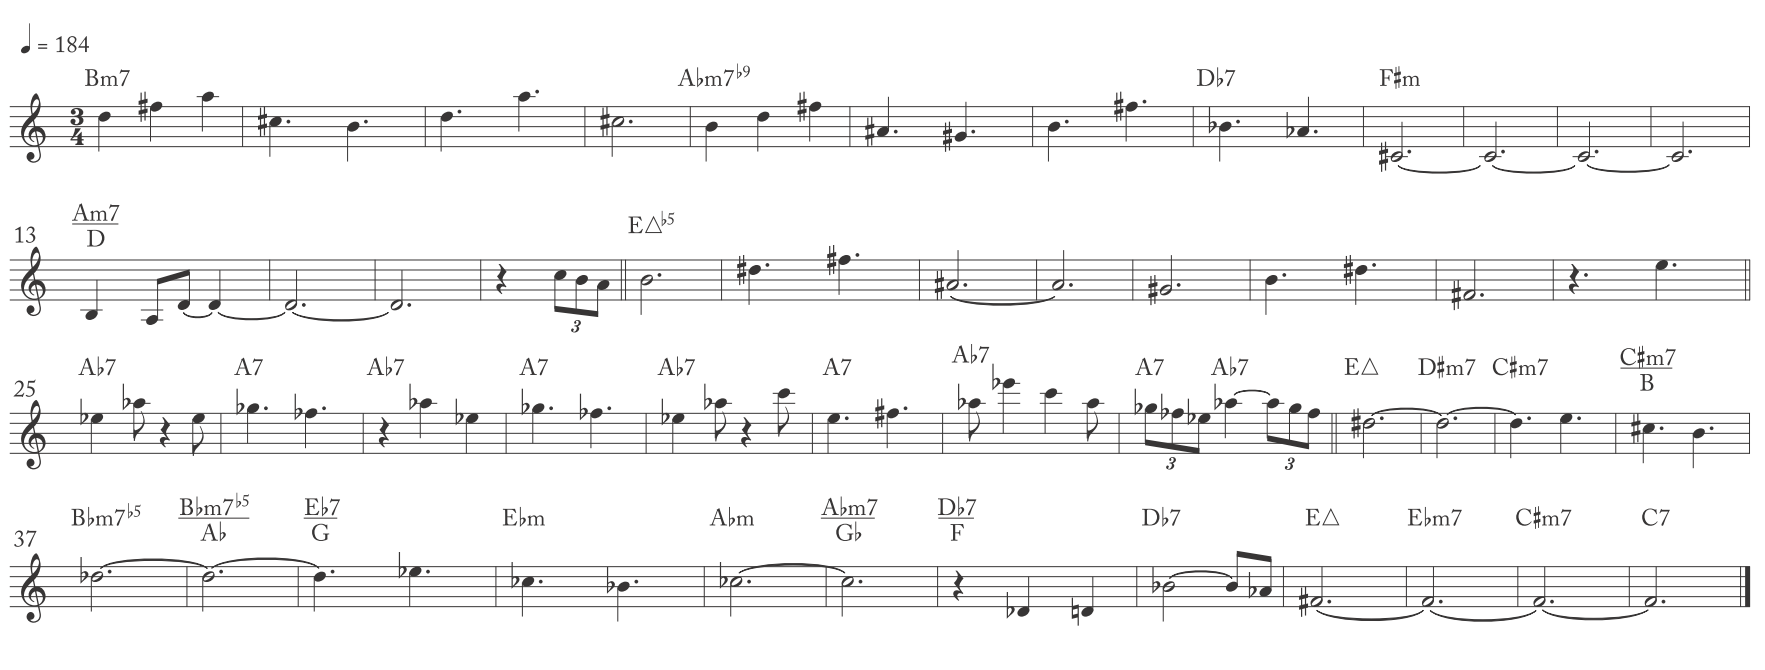
\includegraphics[width=6in]{strunk_windows.png}	
\end{figure}

%Strunk's middleground 1 with extended E prolongation
\begin{figure}
	\centering
	\caption{Strunk's Figure 2, his ``Middleground graph 1" for Corea's ``Windows."  Taken from p.\ 18 of Strunk (2016).}\label{strunk_fig}
	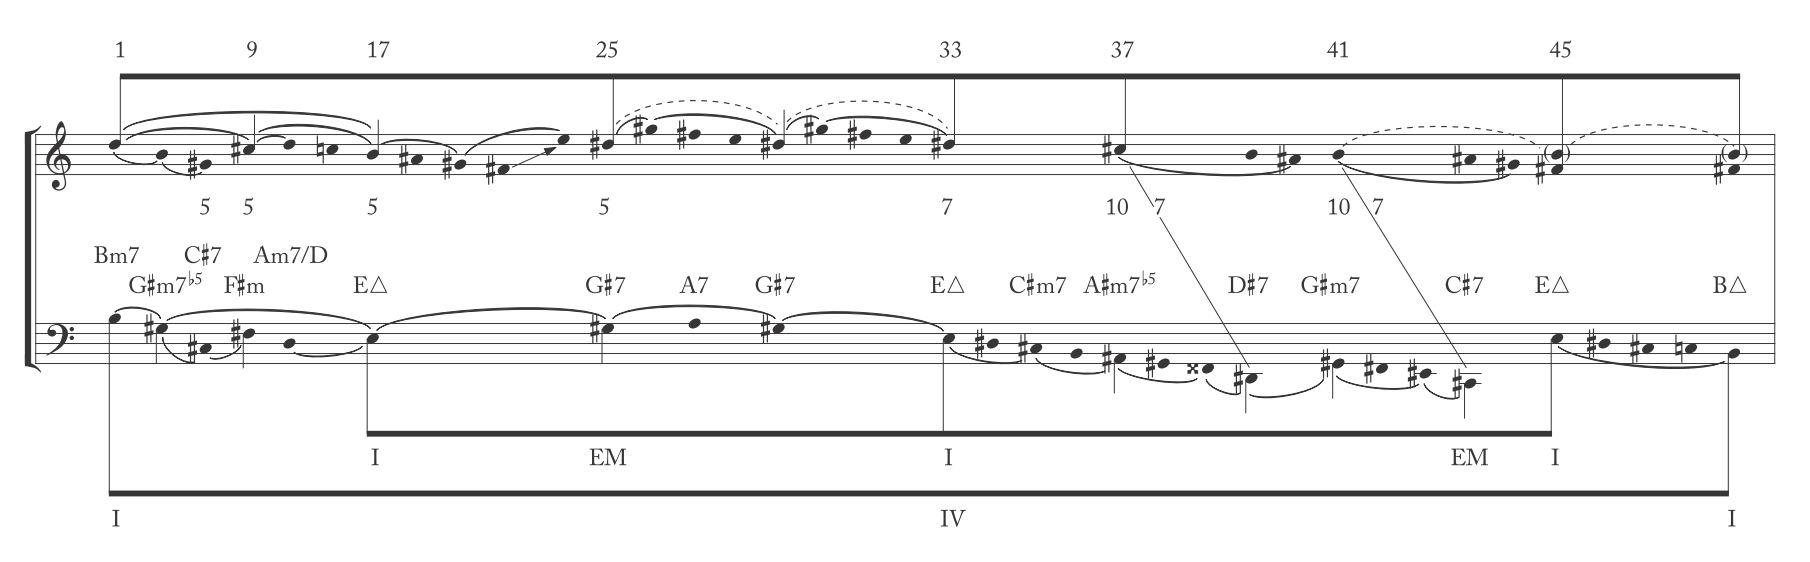
\includegraphics[width=6in]{strunk_windows1.png}
\end{figure}

%Waters
Waters re\"{e}xamines ``Windows" with skepticism regarding the importance of $IV$ as a syntactically functional tonal subdominant, opting instead to describe the piece as a series of ascending fifth-related keys poorly captured by an appeal to the subdominant (or indeed by a monotonal reading in general).  Parsing the tune through the lens of a repeated ascending-fifth ``schema" drawn from Bill Evans's ``34 Skidoo," Waters rehabilitates many of Strunk's embellishing chords as essential stepping stones for a schematic sequence -- $Bm$, $F\sharp m$, $C\sharp m$, $A\flat m$ -- encompassing measures 1-41.  Waters labels the successive ascending-fifth phases of the tune in his Example 2, reproduced here as Figure~\ref{waters_fig}.  Tracing the fifths through the entire tune requires the abandonment, or at least the substantial weakening, of Strunk's $EM$ tonal prolongation.

%Waters's four-stage ascending-fifth schema parsing of Windows
\begin{figure}
	\centering
	\caption{Waters's Example 2, where he parses ``Windows" as a series of ascending-fifth motions.  Taken from p.\ 40 of Waters (2016).}
	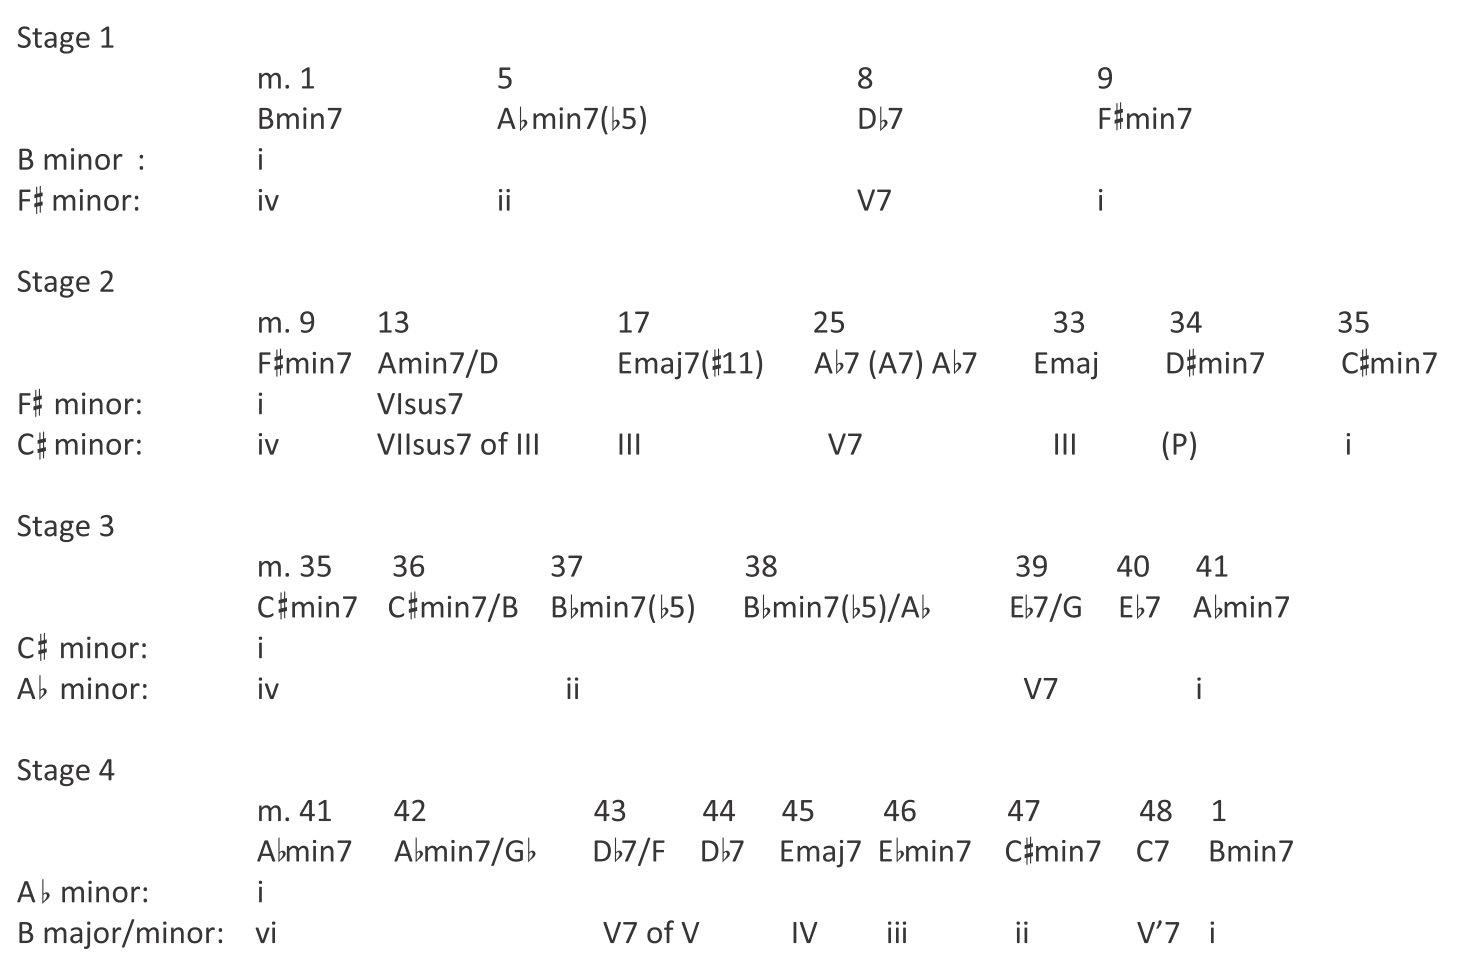
\includegraphics[width=6in]{waters_windows.png}
	\label{waters_fig}
\end{figure}

Waters notes that there are certainly ``compelling reasons" for Strunk's focus on $EM$, including its obvious duration, its hypermetrical placement at the start of two 8-measure phrases, and its appearance at both the beginning and ending of the hypothesized prolongational span.  But here, Waters objects on formal grounds, noting that ``neither duration, hypermetric inflection, nor departure/return is sufficient for prolongation."\footnote{Waters, p.\ 40.}  The usual grounds for prolongation -- presumably, embellishment through common passing or neighbor chords -- are missing, since the prolongation ``is carried out in an unorthodox manner, through $A\flat^7$ (mm.\ 25-32), a harmony in chromatic third relationship with E."\footnote{Waters, p.\ 40.}  Instead, Waters proposes that we hear $EM$ as a relative major substitute for $C\sharp m$, casting his re-labeling as a claim of harmonic relation and temporal delay: ``Thus the mm.\ 33-35 progression EMaj7 - D$\sharp$min7 - C$\sharp$min7 stands for C$\sharp$ minor (with ``stand for" meaning a transformation that meaningfully relates to and delays the more expected C$\sharp$ minor)."\footnote{Waters, p.\ 41.}  If the $EM$ sonorities have a syntactic ``function" in the tune, its primary status is not that of the subdominant of $B$, but rather as a substitute local tonic in $C\sharp m$.

%Waters:Strunk::Wollheim:Loran
I find Waters's analysis rewarding and attentive to the schematic norms of postbop practice, and I will return to his notion of substitutability and ``standing-for" in the next section.  For now, I note that his specific objections to Strunk's analysis echo Wollheim's description and critique of manifest formalism in the work of art critic Erle Loran.\footnote{The Loran discussion comes in \S 12, pp.\ 22-26, of \emph{On Formalism and Its Kinds}.}  In summarizing the argument of Loran's 1943 book on C\'{e}zanne's practice, Wollheim describes a reduction and justification process similar to Strunk's Schenkerian parsing: beginning with C\'{e}zanne's \emph{Still Life with Faience Jug}, reproduced here as Figure~\ref{cezanne}, Loran provides a reductive analytic overlay, isolating and extracting what he sees to be the formal boundaries or outlines of shapes given in the painting.  He then draws ``carry-through" lines designed to track and describe representational, volumetric tension experienced by a viewer.  The two-dimensional outlines give rise to (or represent, or stand as signs for) some phenomenal three-dimensional volumes, and those volumes are relatable to one another in a formal way.  All of this interpretation, Loran states, can be gleaned from the purely configurational (that is, formal, content-free) aspects or indices of the painting.  Wollheim reproduces several of Loran's supporting diagrams, four of which appear in Figure~\ref{loran_diagrams}.

%the cezanne painting
\begin{figure}
	\centering
	\caption{C\'{e}zanne's \emph{Still Life with Faience Jug and Fruit}, from the Oskar Reinhart Collection ``Am R\"{o}merholz," Winterthur.}
	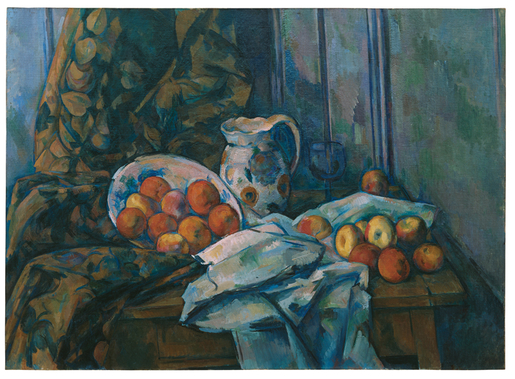
\includegraphics[width=6in]{cezanne.png}
	\label{cezanne}
\end{figure}

%the Loran diagrams
\begin{figure}
	\centering
	\caption{Four of Erle Loran's C\'{e}zanne diagrams, taken from Wollheim (1995), pp.\ 44-45.}
	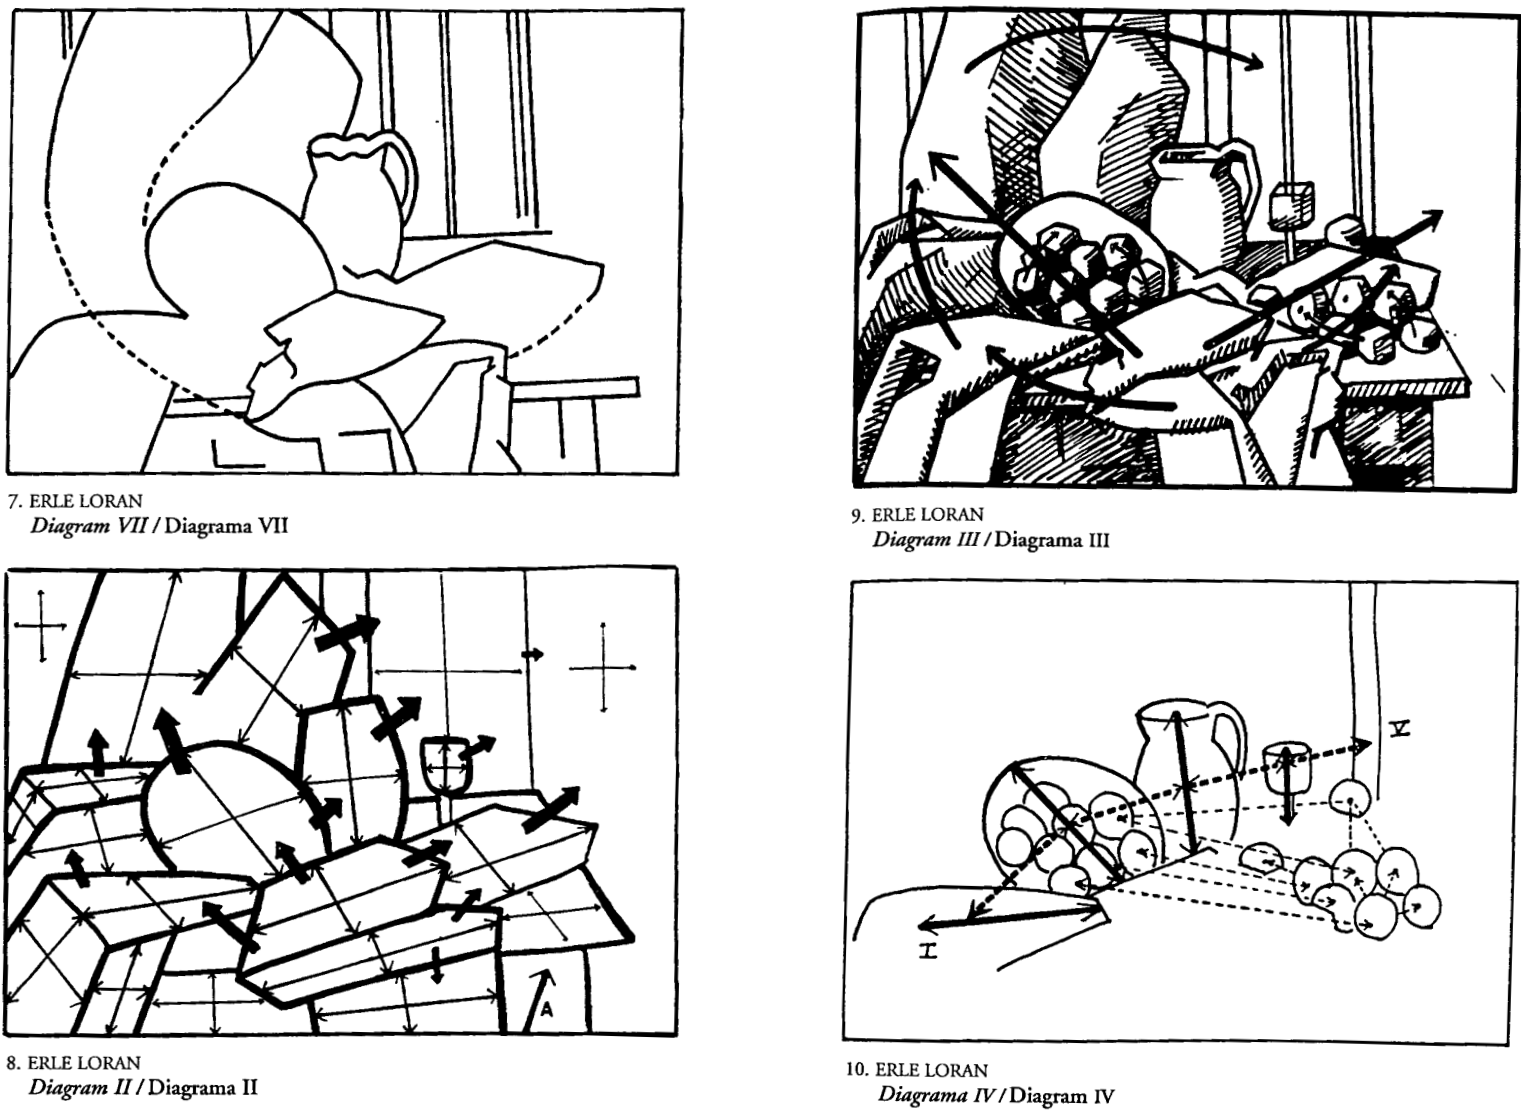
\includegraphics[width=6in]{loran_diagrams.png}
	\label{loran_diagrams}
\end{figure}

Wollheim has two main objections.  First, and more generally, he doubts that the outlines of shapes can be reliably selected from a painting in a consistent and purely formal way, without explicit appeal to the representational content of some viewer.  Judging where a shape begins and ends, Wollheim reminds us, is strongly informed by our internalized norms for the properties of whatever shape(s) and represented object(s) we might recognize in a given visual array.\footnote{Consider Wollheim's discussion of identifying the ``black ring" crowd shape in Breughel's \emph{Christ Carrying the Cross to Calvary} on pp.\ 9-13.}  Second, Wollheim drives a wedge between the two-dimensional outlines and Loran's ``carry-through" lines of three-dimensional tension.  Loran claims that the volumes arise from the formal configurations of the two-dimensional shapes, but Wollheim counters that the moment of turning a two-dimensional array into a represented three-dimensional volume is a psychological one, and that it cannot possibly occur independently of the other (non-formal) aspects of the painting.  As Wollheim puts it in his general rebuttal to manifest formalism, of which he sees Loran's work as a particularly problematic variety,
\begin{quote}
``Observe the earthenware object that lies on the ground on the left-hand side of the picture [Breughel's \emph{Christ Carrying the Cross to Calvary}].  As our eyes alight on it, we recognize it as a domestic vessel.  At this point the beliefs that we have about such utensils confirm us in seeing the dark circle on its body as an aperture opening inwards rather than as a protuberance pushing outwards... [W]e cannot exclude from the formal aspects of the painting any factor that influences what we see in the painting.  And there seems no way in which we can be certain, in advance of particular cases, particular paintings, that some given aspect of a painting will never be such a factor."\footnote{Wollheim, \emph{On Formalism and its Kinds}, p.\ 22.}
\end{quote}
If Loran's three-dimensional tension is meant to arise from ``the similarity in the objects' size, shape, and colour," Wollheim suggests, ``we know better."\footnote{Wollheim, \emph{On Formalism and its Kinds}, p.\ 25.}  Noting visual tension between apples in two different locations in C\'{e}zanne's \emph{Still Life with Faience Jug} seems to involve more than familiarity with outlines and colors.  The identification of representational volumes based on shapes in the visual array, the tensions between those volumes, and even the boundaries of two-dimensional shapes themselves depend on more than just the formal indices of the painting \emph{qua} painting: the viewer's multifaceted visual processing both requires and imposes numerous potentially non-formal aspects for and on any particular ``formal" parsing.\footnote{Wollheim's ultimately psychoanalytic commitment to the process of seeing-in and seeing-as is quite complex, and he would likely resist my use of the term ``parsing," here.  His formalist critiques do not necessarily depend on the adoption of his strikingly Freudian psychoanalytic representational stance, a thorough consideration of which may be found in Whitney Davis's \emph{Queer Beauty} (2010), chapter 10.}

%TODO: this would be one spot for a Kockelman translation of Wollheim.  It could also come after its application to Strunk/Waters.

With the caveat that translation of Wollheim's argument into musical form requires both nuance and skepticism, Waters's response to Strunk can be paraphrased in Wollheim's terms and leveraged toward a paradigmatic critique.  Like Wollheim's manifest formalists, Strunk purports to examine the musical surface and extract (trace) the important harmonies, those that control, prolong, or function as boundaries for tonal spans (shapes).  Reducing away voicings and embellishing chords, Strunk shows an E Major ``shape" as an important formal property of Corea's tune.  With attention to schema drawn from jazz practice, Waters sees a different tonal shape in the passage, and he challenges Strunk's identification of an EM prolongation in a way directly analogous to Wollheim's critique of Loran: Strunk's identification of the formal prolongation seems based on his selection of important musical indices which are, nevertheless, not ``sufficient for prolongation."  To see the shape of the tonal prolongation Strunk identifies, we cannot simply extract surface-level chords to provide a formal justification; like with C\'{e}zanne's apples or Breughel's jug, our identification of the prolongation is dependent on features other than surface harmonic analysis.  If those other features are the ground on which the prolongation rests, no diagram of the type Strunk offers can furnish sufficient proof of its existence.  To put it in Wollheim's words:
\begin{quote}
``Though, through the use of diagrams, [Loran] can analyze, on the one hand, how the artist organizes the picture-plane and, on the other hand, how he organizes the represented space, what, in the nature of things, Loran cannot present diagrammatically is the meeting-point of the two, which is, for him, precisely where C\'{e}zanne's pictorial achievement, indeed pictorial achievement in general, lies... In order to grasp just how C\'{e}zanne fused the organization of volumes and the organization of the picture-plane, we have to go back to the painting itself and experience the fusion: nothing else will do.  There is no formulaic representation of the crucial stage."\footnote{\emph{On Formalism and Its Kinds}, pp.\ 24-25.}
\end{quote}
Since Strunk's prolongational reductions do not represent the moment where the surface harmonies somehow generate or map onto the tonal prolongation he suggests, the prolongation itself can be challenged.  Waters can provide an explanation appealing to a totally different paradigm: the passage might not need to form the shape of a tonal span in the subdominant, but rather could be seen as a series of ascending fifths.

%TODO: here's the other place to put the Kockelman translation of Wollheim/Strunk/Waters
%paradigm comparision, Schenkerian drive-by
The paradigms in play, here, make use of different terms and proof structures-- they start from different ``shapes," and they ``trace" those shapes in different ways.  Strunk's Schenkerian reductions begin with harmonic norms drawn from tonal, western-classical music, and they demonstrate a kind of tonal coherence by selecting surface features from ``Windows" to generate a hierarchy of important tonal features and regions.  Waters's schematic analyses begin with harmonic schema drawn from postbop jazz, and they demonstrate a replicatory chain of influence by interpreting surface voicings in a way designed to show their compatibility with repeated application of the same schema.

%TODO: this is pretty abrupt.  Slow down, expand, work in Kockelman before next section.
The statistical analyses of the preceding chapters cannot reproduce manifest formalist claims of the variety employed by Strunk and other Schenkerian-prolongational theorists.  And while these un-reproduced claims count against a temporal-syntactic paradigm, in one sense, they may be unreproducible for good reason: it may not be possible for data drawn from the surface-level harmonic content of jazz performances to demonstrate Schenkerian claims of tonal harmonic prolongation.  Waters's claims, to the extent that some of them are predicated on parsing jazz progressions in terms of repeated harmonic schema, may lend themselves to a corpus-syntactic paradigm more easily; as such, they (and my own claims) may resemble what Wollheim calls \emph{latent} formalism.

%More on latent formalism/positioning Waters here, or later?
%Might be good to have KW come back after Terefenko, in the heat of latent formalism

\subsection{Functional Analysis as Latent Formalism}
%Finish up Waters as grammatical/quasi-statistical latent formalist
%Terefenko's functions as syntactic latent formalism
%Wollheim's segmentation objection as motivating my project, which doesn't completely solve the problem

%Start with Terefenko-style functional analysis claims
If Strunk's prolongational analysis of Chick Corea's ``Windows" can be described as a kind of manifest formalism, as my Wollheimian extension of Waters's response implies above, it stands as one type of claim regarding jazz harmony unreproducible under the corpus-syntactic paradigm of chapters 2-4.  Manifest formalism does not exhaust the space of unreachable claims, however; two other paradigmatic modes of discourse on jazz harmony seem not to find a statistical home -- pedagogical approaches and functional analyses of individual tunes or performances.  As an exemplar for both of these varieties of inquiry, I turn below to Dariusz Terefenko's \emph{Jazz Theory: From Basic to Advanced Study} (2014).  I aim to unpack Terefenko's textbook partly as a latent formalist project, in Wollheim's terms, and I will ultimately suggest that my own work inclines in this direction, as well.

Terefenko does not aim his book at music theorists, at least not directly; rather, the text is meant for dedicated, adventurous musicians, ``undergraduate and graduate jazz students, and for an ever-increasing population of classical students interested in jazz theory and improvisation."\footnote{Terefenko, p.\ xv.}  As such, the book takes a fair amount of western-classical theoretical assumptions as a ground, providing quick primers on scales, meters, triads, and roman numeral analysis designed as reminders rather than explicit theoretical claims.  Since Terefenko presents theory in the service of practice, I will not subject his claims to quite the same critical attention as those in theoretical works like Strunk's or Waters's.  But attending to the model implicit in most of the book will, nevertheless, clarify one of the major presentational paradigms in jazz pedagogical literature.\footnote{For other, similarly latent-formalist and pedagogical examples, see ?????}

While Terefenko's descriptions for phrase models and song forms presented in Part Three invoke Schenkerian techniques, the earlier portions of the book treat prolongation with a light touch, instead presenting a wide array of chords through the lens of functional categories.  Terefenko describes harmonic function quasi-grammatically from the outset:  after introducing tonic, predominant, and dominant as the necessary components (or ``contextual features") of functional tonality, he describes their interrelated tension and release patterns in traditionally energeticist ways.\footnote{Cite the history of such quasi-psychological energeticism?  Halm or Kurth, Rothfarb 1992?}  The restful stability of the tonic, the moving-away of the predominant, and the tense instability of the dominant are all ``different behavioral patterns," which ``remain constant across the entirety of the tonal system in which jazz forms a distinctive musical language with its own harmonic grammar and melodic syntax."\footnote{Terefenko, p. 26.}  But even as Terefenko firmly grounds jazz harmonic function within a western-classical tonal paradigm, he makes space for its own idiomatic dialect: ``As will be demonstrated time and time again, functional tonality in jazz has different properties than that of common-practice classical music.  These properties are represented by a unique set of rules dictating the unfolding of harmonic function, voice-leading conventions, and the overall behavior of chord tones and chordal extensions."\footnote{Terefenko, p.\ 26.}  Much of the rest of the book is dedicated to stipulating these rules and showing examples of jazz harmony's idiomatic grammaticality.

%Use Wollheim to describe them as latent formalism
As Terefenko assigns a plethora of jazz chords to the three basic functional categories, he builds the lexicon of a complex grammatical system with a comparatively simple syntax.  The tonic, predominant, and dominant, which exist as idealized parts of musical speech, occur in a small number of grammatical orderings; most of the interest in jazz harmony, for Terefenko, consists of complicated mappings from increasingly dissonant chords to their interpretive functional categories.  Parsing musical surfaces toward this end produces what Wollheim would call a latent formalist system, where the harmonic drama arises from the underlying syntax of progressions.  Wollheim offers an extremely clear description of linguistically-inspired latent formalist models, claiming that rules of syntactic organization must meet five requirements:
\begin{quote}
(one) they presuppose some way in which larger units can be segmented into smaller units, and ultimately into basic units;

(two) they then operate on the basic units, which they first classify under certain general categories.  In the case of language, examples of such categories are noun, verb, adverb;

(three) they order these elements, classified by category, into strings of elements that are well-formed, or grammatical, while all other strings are ill-formed, or ungrammatical;

(four) the rules function recursively, in that they can be endlessly reapplied to their own output so as to yield an unbounded set of further well-formed strings; and

(five) in those cases where the strings refer, or have a semantic dimension -- that is, in all cases except purely formal languages -- the meaning that each string has is determined by its syntactical form plus the vocabulary, or lexicon, of the language.\footnote{Wollheim, pp. 26-27.}
\end{quote}
Terefenko's functional harmonic syntax engages with each of these requirements.  He explicitly states that passages of varying length can carry functions or be divided into elements which do so; he classifies those harmonic elements into functional categories; he deploys the elements (usually chords) in well-formed progressions, repeatedly and with variation.  If Terefenko's musical strings (usually harmonic progressions) do indeed refer, along the lines of Wollheim's fifth requirement, their semantic dimension might encompass a particular tune or style of playing, both of which are presumably recognizable from the combination of functional syntax and a particular lexicon, be it voicings or head changes.  But setting aside musical semantics, a proper analysis will reveal the hidden (latent) syntax of a given passage, and a proper composition will follow the grammatical production rules for ordering categories to produce an intelligible tune or improvisation.

For formalist projects of this general type, Wollheim offers another critique.  Taking to task Yve-Alain Bois's semiological description of Picasso's Cubism, Wollheim shows that a supposedly-syntactic analysis of Picasso's \emph{Head of a Girl} or Grebo mask must fail to satisfy the requirements given above.  Three of Wollheim's objections find possible counter-arguments in Terefenko's syntax.  Wollheim claims that Bois ``proposes no categories analogous to those of grammar," while Terefenko does; Bois offers no rules for how to concatenate categories, while functional harmony does this, in a general sense; and Bois offers no sense of what un-grammatical works of art might be: ``He gives us no reason to think that pictorial objects can be divided into the well-formed, which are legitimate, and the ill-formed, which are illegitimate, where this division is effected on the basis of whether or not rules of a very specific kind have been properly applied in their production."\footnote{Wollheim, p.\ 30.}  If one of Terefenko's students is expected to improvise with other musicians and write tunes in a mutually-understandable idiom, there may well be social and grammatical norms separating well- and ill-formed utterances.  Terefenko's functional harmony avoids many of Wollheim's latent formalist objections.

Terefenko's functional syntax may not, however, satisfy one of Wollheim's objections:  Wollheim complains that Bois offers ``no systematic way in which the total surface of the pictorial object could be segmented-- segmented, that is, without remainder-- into parts, which could then function as syntactical constituents."\footnote{Wollheim, p.\ 29.}  When confronted with a complex visual array, a Boisian latent formalist must somehow decide both how to chop up the painting into syntactic elements and how to recognize each element as part of the appropriate grammatical category.  This segmentation difficulty has an auspicious musical history in atonal music theory,\footnote{See some citations of the segmentation problem inherent in pc-set theory.} but it applies to Terefenko's contextual parsings, too.

As one parsing example among many, consider the simple tonal progression on his p.\ 33, reproduced here as Figure~\ref{Terefenko_ex}.  For Terefenko, several of the chords can be given \emph{a priori} functional assignments based on their pitch structure -- in the limiting case, Terefenko has given the student no category other than tonic for the minor $i$ chord, but $V$ and $ii^\circ$ also seem unambiguous, here.  The $VI$ chords of measures two and four, however, merit special consideration:
\begin{quote}
The third chord of the progression, the submediant also has two functional assignments: tonic and predominant.  Based on the surrounding context though, especially the forthcoming $iv$, the $VI$ can be interpreted as belonging to the predominant family of chords.  The predominant $ii^{\circ}$ in m.\ 3 forms a cadential gesture with the dominant that then resolves deceptively to the $VI$.  Given the two functional assignments of $VI$, it functions as a tonic in the context of this progression.
\end{quote}

\begin{figure}
	\centering
	\caption{Terefenko's Figure 3.10, a tonal progression in minor.  Each chord receives a roman numeral based on its pitch structure, and Terefenko employs a multi-level parsing to assign functional categories to each roman numeral, starting from the clearest cases and extrapolating to ambiguous ones.}
	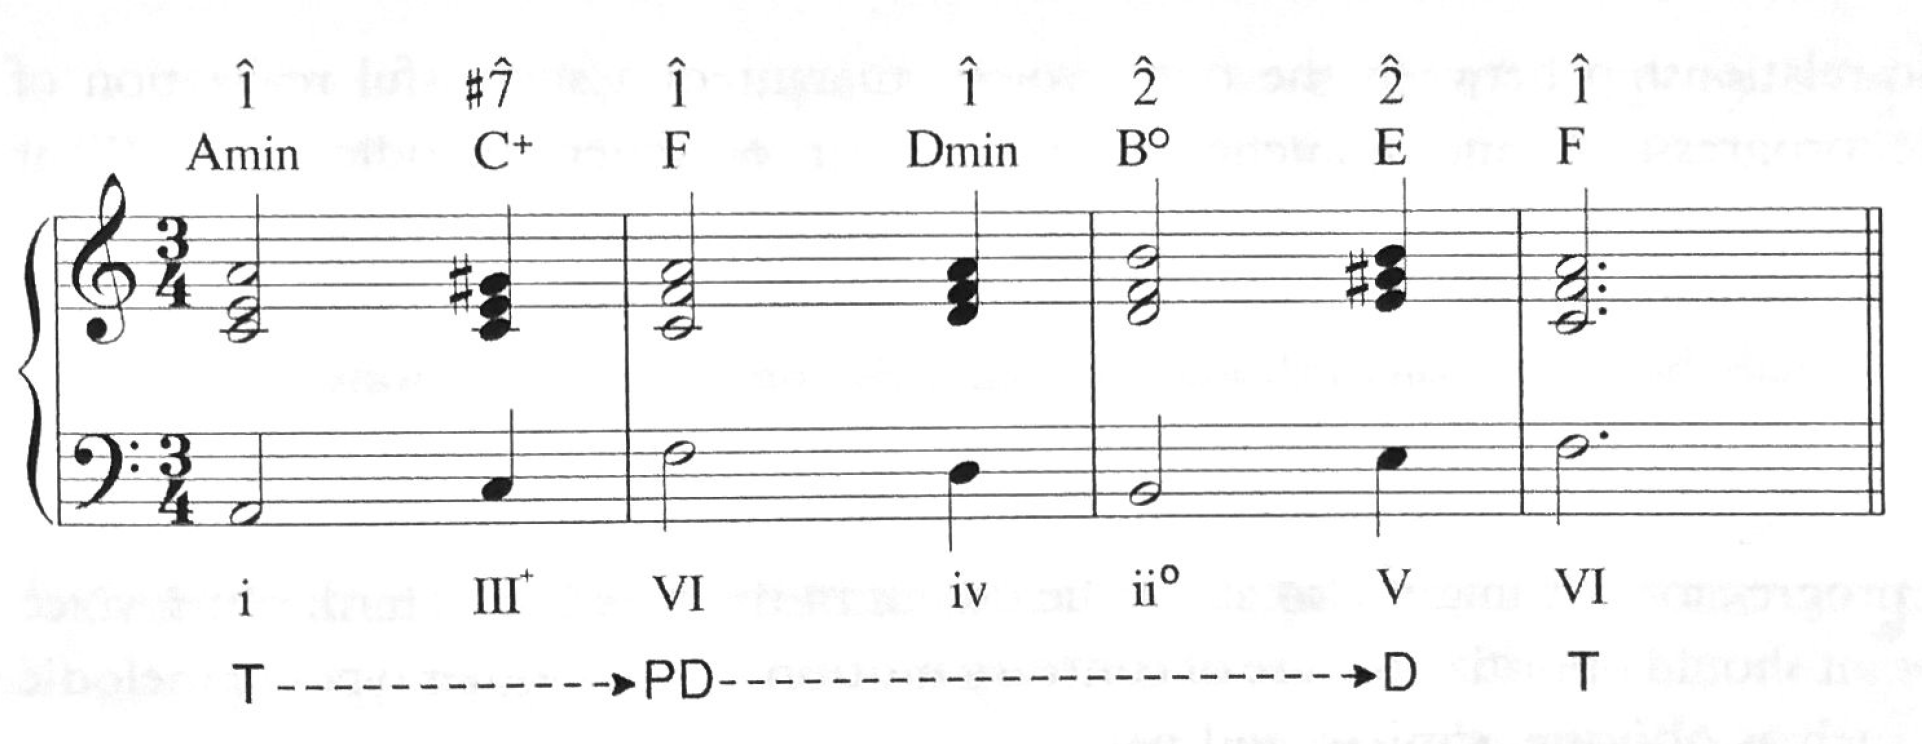
\includegraphics[width=5in]{Terefenko_ex.png}
	\label{Terefenko_ex}
\end{figure}

The segmentation procedure Terefenko employs is sensitive and emblematic of latent-formalist jazz analyses: begin by assigning a rooted, tertian-stack roman numeral label to each sonority, and consult a table of functional assignments to determine the category to which each roman numeral belongs.  When the category assignment is ambiguous, fall back on the local context of the phrase, tracing a quick hermeneutic loop designed to produce whichever functional label best fits the analyst's expectation for normative behavior in the local context.  In Terefenko's words, ``The surrounding harmonic context in which chords occur determines the analytical interpretation of these chords."\footnote{Terefenko, p.\ 33.}  If that is true, then the assignment of particular chords to functional categories does not depend (or, more charitably, does not \emph{only} depend) on their pitch structures, despite the fact that the rest of Terefenko's material on harmonic function makes repeated reference to pitch-based tables of harmonic functional categories.  The implied segmentation procedure is not \emph{a priori} consistent, and it requires foreknowledge of which contextual forces will override the pitch-based category assignments found in elementary descriptions of tonic, predominant, and dominant.

This hermeneutic circle at the heart of functional parsing renders harmonic analysis flexible and fertile, but it also renders any truly latent formalist system incomplete or circular.  If there is no explicit account given for how functional assignment is to be accomplished without recourse to the analyst's expectations, the formalist parsing runs the risk of confirming any preconceptions the analyst has.  As I claimed in Chapter 1's discussion of Lerdahl \& Jackendoff -- also latent formalists, much more explicitly -- the ``rules" of syntax cannot be proven on the basis of analyses of this kind, as contextual parsing will allow the analyst to shoe-horn a wide variety of musical surfaces into the analyst's pre-existing theory of harmonic syntax.  Terefenko is able to avoid an explicit framing of functional category assignment precisely because the paradigm under which he operates assumes one implicitly: the pedagogical analysis of particular passages implies a set of top-down ``rules" to be taught to the student, and the application of those rules results in claims about the music at hand.  Whether those claims are meant to encompass how the teacher hears the music, how the student ought to hear the music, or something about the structure of the music independent of a hearer cannot readily be determined within the paradigm's framework.%last part of this paragraph is weak

%Wollheim's objection motivates my project
Latent functional analysis for pedagogical purposes may yet be re-writable under a temporal syntactic paradigm, but Wollheim's segmentation objection must first be dispatched: the data-driven temporal segmentation and clustering performed in chapters 2-4 is an attempt to do so.  Where Bois cannot separate elements within the Grebo mask, chapter 2 suggests that voicings or scale-degree sets might be extracted from YJaMP based on their temporal properties -- that we can consistently partition the notes of a performance based on the perplexities of time-window note distributions and statistical patterns of inter-onset timing.  Where Bois cannot give an account of what general categories of syntactic behavior might exist for elements of the mask, and where Terefenko assumes pre-existing western-classical functions, chapter 3 suggests that statistics regarding temporal behavior on different time scales can serve as a ground for a kind of syntactic functionality.  And where Bois cannot provide meaningful rules assigning elements of the mask to syntactic categories or ordering them, Terefenko relies on hermeneutic application of western-classical functional patterns.  Chapter 4 suggests that clustering chords based on similarities in their PCA-reduced temporal properties provides a starting point for functional assignment independent of many analytical pre-conceptions, but the process described there accomplishes a task quite different from  Terefenko's harmonic parsings.  Unlike Wollheim's art-theoretical critique, a corpus of jazz piano harmony permits linguistically-inspired latent formalist description accountable to musical data.  Whether the resulting description still permits productive hermeneutic engagement with individual tunes for students and analysts is an open question.

\section{Paradigmatic framings}
%kockelman here, and use it to reframe the historical and latent formalism above
Wollheim's objections to manifest and latent formalism survive (or benefit from) translation into semiotic ontological terms. Pulling his criticisms apart across Kockelman's semiotic diagrams allows the specification of blocked or successful channels of communication between agents, stable or unstable objective ontologies, and interpretants produced through parasitic means.  With these framings in hand, I will be in a position to suggest what kind of semiotic processes the corpus analytical pipeline of chapters 2-4 affords; the resulting latent formalist framing co-generates objects and analysts well-aligned for only certain modalities of syntactic interpretation.

\begin{figure}
	\centering
	\caption{Formalist parsings implied by Loran and Strunk (top) as subject to critiques by Wollheim and Waters (bottom).  Both criticisms may be thought to split and re-frame the parsings into chains of semiotic processes.}
	\label{critiques}
	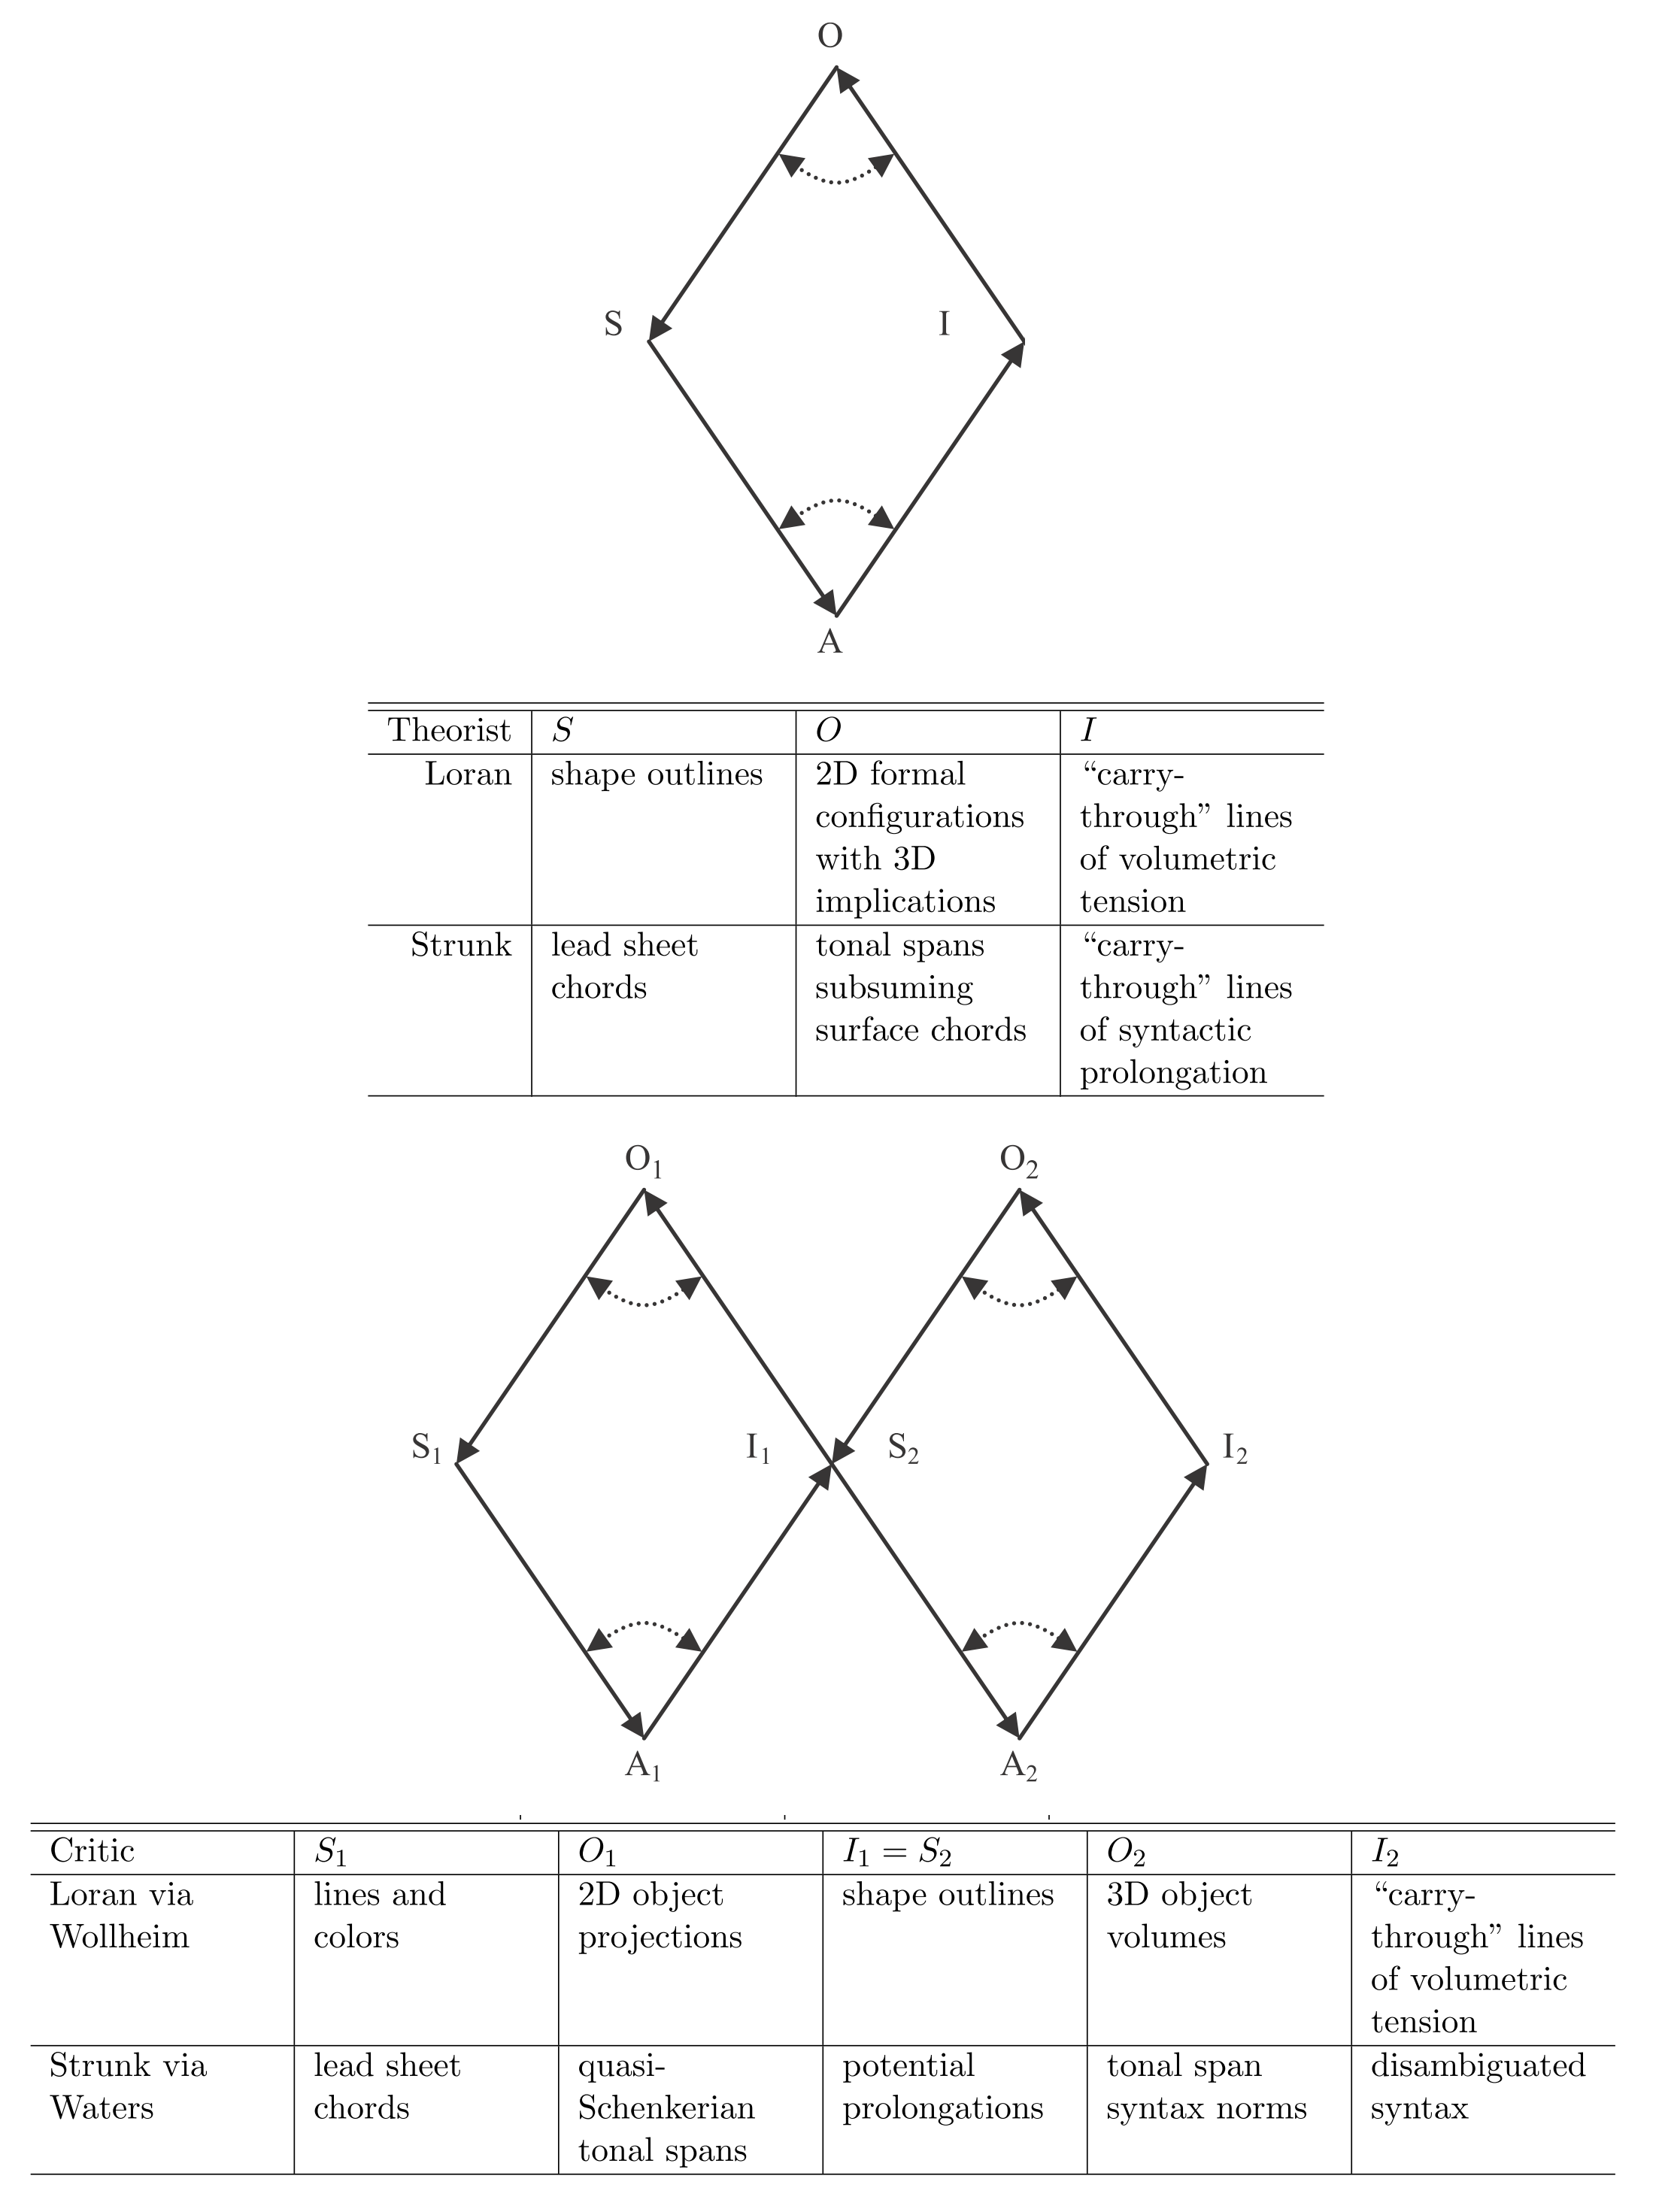
\includegraphics[width=6in]{critiques.png}
\end{figure}

The top half of Figure~\ref{critiques} provides one possible framing for the formalist analyses of Loran and Strunk.  In broadest strokes, each mode of analysis purports to begin with surface features, indices $S$ directly sensible by the analyst $A$.  As Loran would have it, these are two-dimensional shape outlines observable on a painting; for Strunk's analysis of ``Windows," these indices are the chords of the published lead sheet.  Both analysts interpret these indices as signs standing for some kind of object ($O$), and they produce analytical interpretants ($I$) meant to make sense given its properties.  Both produce graphical interpretants (which often serve as indices for other semiotic processes): Loran's ``carry-through" lines of projected volumetric tension and Strunk's tonal syntactic prolongations.  Coincidentally, both use roman numerals as part of their interpretants.  More consequentially, both give meaning to their interpretants with both the observed indices and the properties of spans, objects, or configurations not identical with the observed surfaces.

For Loran to turn shape outlines into carry-through lines, his actions necessitate the existence of objects with two-dimensional formal configurations and three-dimensional volumetric implications -- only in light of both of these kinds of property can the relation of $I$ to $S$ make sense for $A$ (Loran).  For Strunk, prolongational sketches only make sense given the existence of mostly-Schenkerian tonal spans subsuming surface chords.  These spans have some surface chords as observable indices, but the carry-through lines do not merely identify the repeated appearance of those indices -- rather, they make sense given some aural, psychological, or acoustic properties of the tonal span objects.

Wollheim's challenge to Loran and Waters's critique of Strunk appear in the bottom half of Figure~\ref{critiques}, where I interpret each critique as a further specification of (two of) the multiple semiotic framings involved in the production of Loran and Strunk's interpretants.  Wollheim doubts that the formal configuration objects produced by Loran's framing can arise from or connect to the indices of the paintings in a reliable (and representation-free, as Loran would have it) way.  He pulls apart the identification of shapes, noting that Loran really sees lines, dots, colors, shades, and so forth ($S_1$), not shape outlines. He must first interpret those indices as shape outlines -- and an analyst doing so will almost certainly make explicit or implicit reference to his or her experience with the two-dimensional projections of objects in the world.  Tracing a pot-shape involves recognizing a pot; it is not na\"{i}ve.\footnote{I note in passing here that an algorithm \emph{could} trace a pot without any possibility of knowing what it ``is."  In that case, the interpretant produced by the tracing algorithm (that is, the ``shape") would make sense given the properties of a different class of object with a different ontology -- not shape-schema drawn from objects in the world, but some specifications encoded in the algorithm (like recognition of lines and colors, continuity and discontinuity, and so forth).  An algorithm identifying a shape might produce a similar-looking interpretant to a human identifying the ``same" shape (i.e., ``CIRCLE"), but the two are imbricated in quite different semiotic structures.  The price of the consistency offered by the algorithm is that it may not serve ends a human would pursue.  This leads directly to considerations of semiotic parasitism, as will return below at more length.} The analyst then interprets these shape outlines ($I_1 = S_2$) in order to produce lines of volumetric tension which make sense given the properties of three-dimensional objects in general ($O_2$).

In a framing of this kind, Kockelman often notes that the relation between $A_1$ and $A_2$, the agent performing each of the analytical tasks required of Loran, is mediated by the relation between the objects they are selecting and signing, $O_1$ and $O_2$.\footnote{For example, see the semiotic discussion of Aristotelian and Marxist ``social relations" on p.\ 38 of Kockelman 2012, ``a relation between people mediated by a relation between things, where both these modes of relationality are themselves grounded in significance and selection."}  For the production of shape outlines to be purely formal, or based only on the configuratedness of the painting, $A_1$ should not consider three-dimensional properties of particular things in the world $O_2$ -- those are emphatically not indices observable on the painting's surface.  But while the signed objects $O_1$ have two-dimensional surface properties recognizable as shape outlines, Wollheim notes, interpretation of their shapes is impacted by exactly that knowledge (that is, the properties assumed by $O_2$).  The communicative relation between the analytical agents of the two framings (be they unconscious psychological processes or Loran in two conscious modes of analysis) is transacted through and mediated by the relations between these objects.  If $A_2$ cannot accomplish its tasks based purely on the painting's formal indices, neither can $A_1$; and if the properties of $O_2$ can determine the properties of $O_1$, then so can the representational analyst $A_2$ exert authority over the ``formal" parsings of $A_1$.

As explicated by Waters, Strunk's implied manifest formalism involves a similar framing.  The prolongational identification in ``Windows" is accomplished by selecting musical surface indices $S_1$ and using them to identify tonal spans $I_1$.  As Waters points out, this identification is, on purely formal terms, underdefined; some surface indices support it, like metric and hypermetric placement, but no obviously Schenkerian harmonic elaborations appear. Since no formal span-identification underpins Strunk's prolongations, several possible spans might be identified ($I_1$).  These spans then serve as indices for another process, by which Strunk must decide that the syntactic context of one particular prolongation makes it more probable -- more well-formed, in linguistic terms -- than other possibilities.  Agent $A_2$ employs a kind of syntax norm to turn potential prolongations into the final syntactic analysis Strunk offers, while agent $A_1$ is meant to rely on purely surface features ($O_1$).  Again, the $O_2 \rightarrow O_1$ relation mediates the $A_2 \rightarrow A_1$ relation: the identification of the prolongational spans cannot be accomplished based only on surface features, but rather is informed by pre-existing expectations regarding harmonic syntax.  This is not disqualifying, especially since Strunk's expectations largely align with those of other experienced jazz analysts.  Waters, however, suggests an alternative: well-formed, syntactic spans in post-bop jazz might have different schematic norms from Schenkerian prolongations (say, $O_{2^{\prime}}$), which might have a different influence on the properties of tonal spans ($O_{1^{\prime}}$).  The identification of tonal prolongations does not provide a proof of Strunk's functional parsing, since that identification already involved a particular semiotic communication between related agents -- and other types of syntax might align with or determine other types of ``prolongation."

As he lays out the case for a repeated-schema parsing of the syntax in ``Windows," Waters frames a pair of semiotic processes relying more explicitly on latently syntactic categories of temporal progression behavior.  From lead sheet chords, Waters produces potential schema segmentations $I_{1^{\prime}}$ which make sense given the properties of schema ($O_{1^{\prime}}$), which have particular surface chord indices and repeat in time.  Ambiguous schema segmentations are then adjudicated ($A_{2^{\prime}}$) by analytical appeals to categories of syntax-preserving chord substitutions ($O_{2^{\prime}}$).  If ``the mm.\ 33-35 progression EMaj7 - D$\sharp$min7 - C$\sharp$min7 stands for C$\sharp$ minor," as Waters writes, it must bear some similarity to it. Waters describes his semiotic standing-for as ``meaning a transformation that meaningfully relates to and delays the more expected C$\sharp$ minor."\footnote{Waters, p.\ 41.}  The temporal context in which the progression appears both permits and modifies a statistically-normative syntactic progression.  These considerations still impact the selection of schema accomplished by $A_{1^{\prime}}$ in a way not \emph{a priori} better or worse than Strunk's framing.  A different semiotic pipeline connects the syntactic disambiguation to the musical surface, and it employs objects with different properties to segment the surface and assess its well-formedness.

%transition to Terefenko and latent formalism
These analytical programs rely on the production and identification of spans with particular surface and non-surface properties, a kind of tonal hearing-as relying on a complex communication between segmentation and expectation.  But even syntactic projects which do not directly invoke spans implicate similar semiotic processes.  Before diagramming the affordances and limitations of the pipeline given in chapter 2-4, I frame Terefenko's parsing as emblematic of latent-formalist syntax in harmonic analysis pedagogy.

%Terefenko
Figure~\ref{k_t} diagrams my interpretation of the pipeline from the musical surface to Terefenko's syntactic parsing labels.  In the leftmost diamond, Terefenko's chord analyses first turn vertical pitch stacks $S_1$ (that is, chords which could be notated in a score) into roman numerals $I_1$.  Like Strunk's parsing, Terefenko's roman numeral assignments start with the pitch contents of a given verticality; unlike Strunk's parsing, prolongations play no clear feedback role in labeling.  All that is required, for Terefenko, is that the verticality have a clear key-relative root and appear roughly tertian, though he allows sophisticated chord-structural alterations later in the book.\footnote{Note that the explanation for adding new structures to a roman numeral category is almost always functional -- the added chord ``behaves like" a member of the category -- despite the pitch-based, context-free origin of the categories.}  When assigning a roman numeral, the agent/analyst $A_1$ knows only the key and the pitch structure.

%TODO: does T justify his categories with content provisions?
Next, Terefenko turns roman numeral labels ($S_2$) into possible functions $I_2$ (for him, usually $T$, $PD$, or $D$).  When parsing a particular tune or passage, this consists of consulting a table of typical roman numeral functions -- sets of roman numerals Terefenko deems syntax-preserving.  A single roman numeral might belong to more than one category of syntactic function (like $VI$), and the initial identification of these categories is purely content-based.  Indirectly, of course, the categories reflect progression tendencies, but the production of potential functional assignments $I_2$ only depends on the existence of syntax-preserving categories $O_2$, however they are formed.

As in the parsing of Figure~\ref{Terefenko_ex}, these content-driven functional assignments require disambiguation.  $A_3$ accomplishes this by applying conditions of syntactic well-formedness to the surrounding (and especially following) chords of the local phrase or referential tune.  Considering each of the possible syntactic functions $S_3$, Terefenko recognizes that other, less-ambiguous nearby functions may support one choice over another.  Given the existence of syntactically well-formed progressions, $A_3$ produces a disambiguated syntactic parsing $I_3$.  What enables communication across these processes?

\begin{figure}
	\centering
	\caption{My framing of Terefenko's contextual syntax parsing as three semiotic processes in communication.  Dotted lines (\textbf{a}) and (\textbf{b}) indicate the close relations between the significant properties of $O_1 / O_2$ and the selecting actions of $A_1 / A_2$.  Dotted lines (\textbf{c}) and (\textbf{d}) indicate relations between the categorical objects $O_2 / O_3$ and the analytical agents $A_2 / A_3$.  All of these relations between relations are implicated across signed indices $S_i$ and instigated interpretants $I_i$.}%DENSE caption
	\label{k_t}
	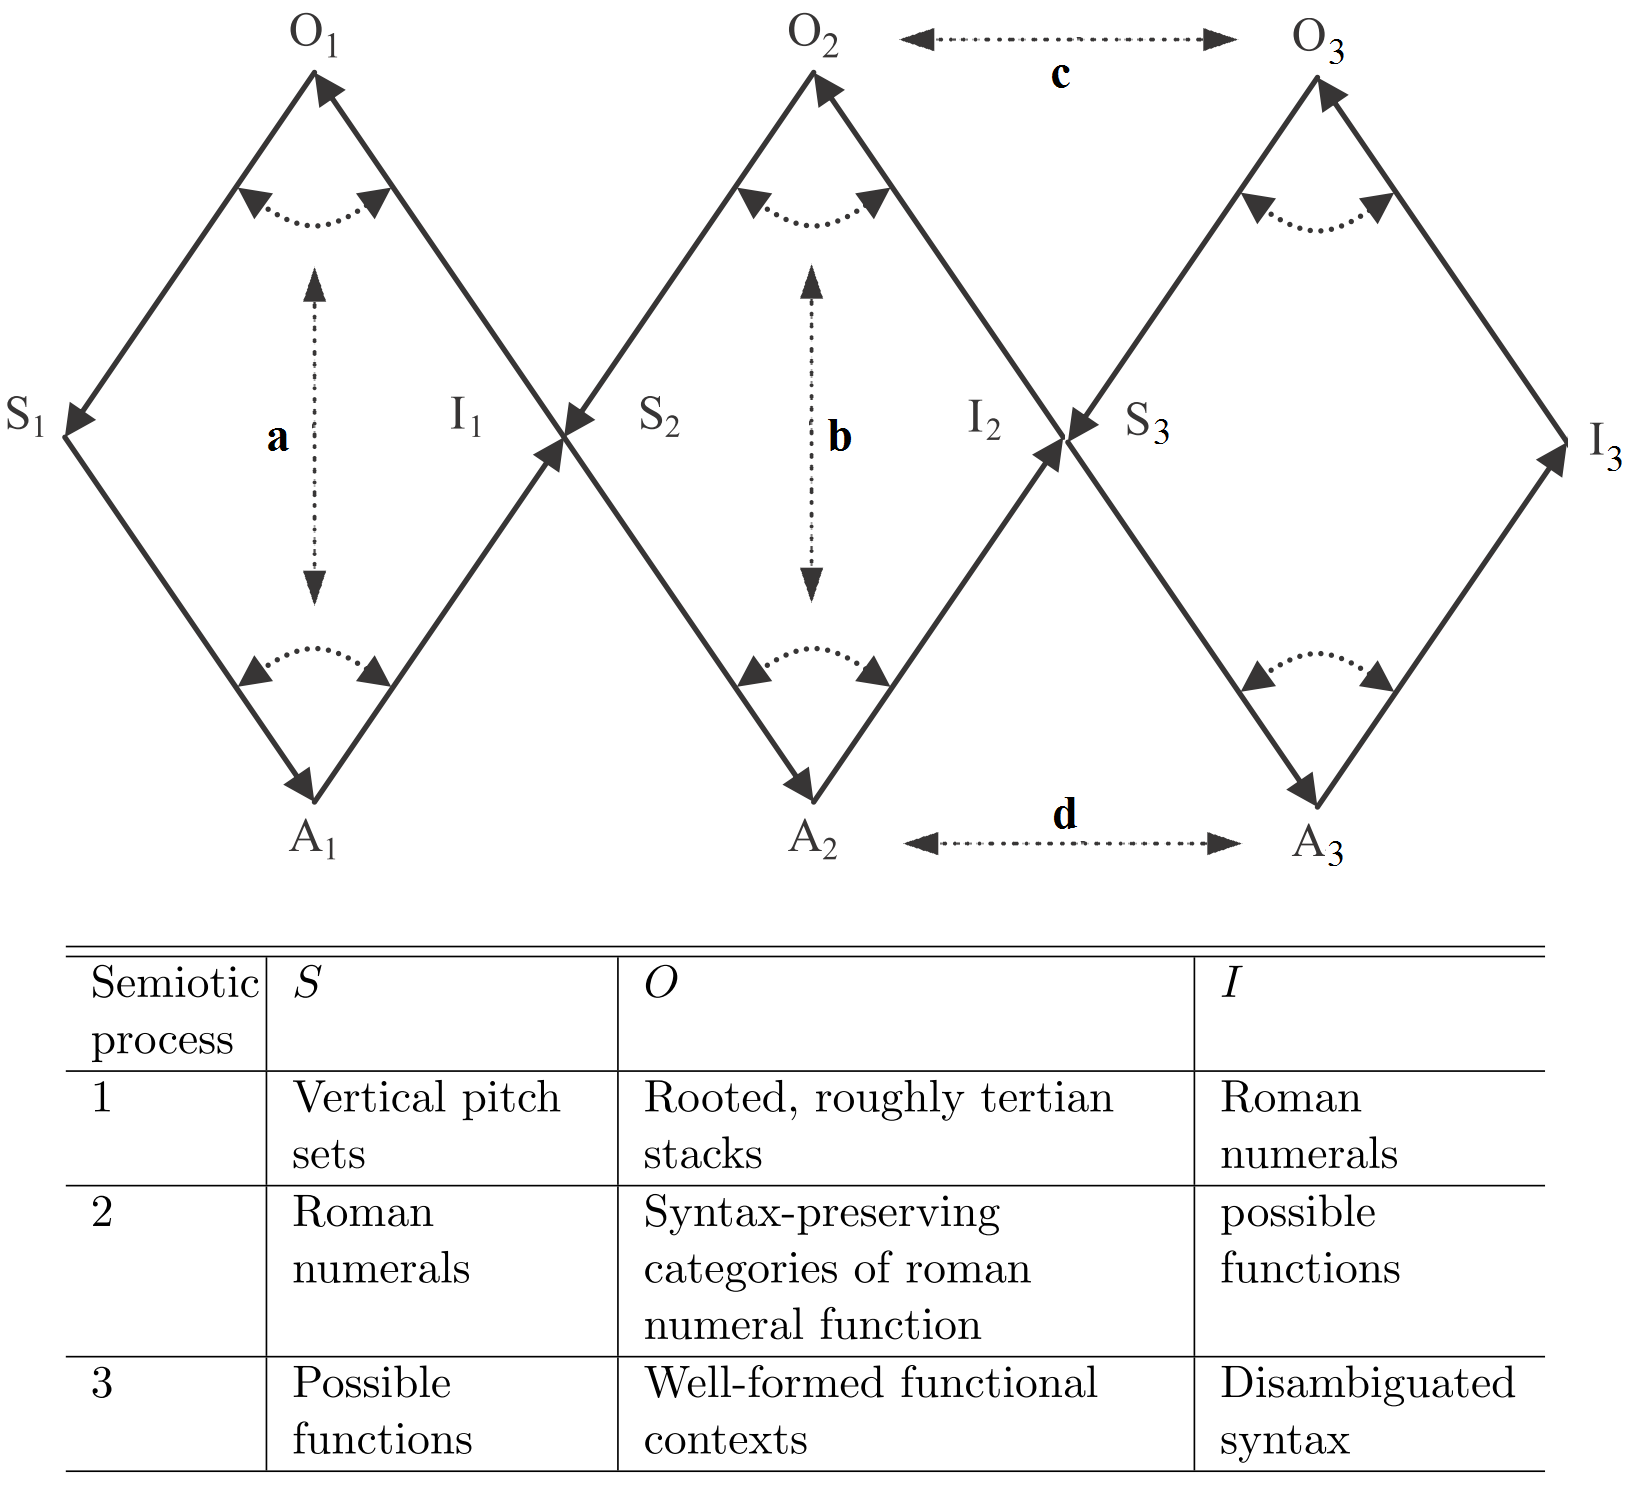
\includegraphics[width=6in]{kockelman_3simple.png}
\end{figure}

The dotted lines on Figure~\ref{k_t} denote the relations between relations underpinning (and undermining) semiotic communication.  First, as in the standard Kockelman framing, the properties and indices of the objects $O$ and the knowledge and actions of the agents $A$ make sense in complementary ways, as indicated by arrow (\textbf{a}).  The assignment of roman numerals $I_1$, for example, makes sense given the significant properties of $O_1$ only if the local pitch indices $S_1$ sign categories of key-rooted chords; the categories only have such indices by virtue of their selection by the agent.  Arrow (\textbf{b}) may describe a directly analogous process, where the identification of potential functions $I_2$ makes sense given the significant properties of $O_2$ -- that syntactic categories are indexed and signed by roman numerals.  Since the roman numeral label $I_1$ arose from content-driven analysis, with verticalities standing for their pitch-identified categories, $A_2$ may relate to $O_2$ in the same way (and with the same immediate ignorance of contextual or temporal information other than key).  The agents communicate across $S_1 \rightarrow I_2$ by virtue of this semiotic channel, where indices sign categories of verticalities.%TODO: check where Kockelman discusses channels?

From the right hand side of the diagram, channel comparison can be run in reverse.  $A_3$ cannot examine the potential functions $I_2 = S_3$ atemporally; without context, there is no way to determine whether or not a functional assignment will result in well-formed syntax.\footnote{Even in the limited string-matching case for well-formedness rules, where this might be done through examining a table of acceptable function strings, their \emph{ordering} must matter and will encode directly temporal properties into $O_3$.}  The properties of well-formed contexts explicitly require temporal progression indices, orderings of functions in time, to narrow down the potential assignments to one syntactic label $I_3$.  But if the $A_3 \rightarrow A_2$ relation (arrow (\textbf{d})) is mediated by the $O_3 \rightarrow  O_2$ relation (arrow (\textbf{c})), the different ontological conditions of the object categories necessitate strongly differentiated analytical interpreters.  Conversely, if the agents share goals, methods, or communicative channels, the resulting close relation $A_3 
\rightarrow A_2$ implies that the ontologically-(non)distinct categories $O_2$ and $O_3$ will inform one another.

I claim that syntax-preserving categories of roman numeral function $O_2$ are systematically over-determined, both for Terefenko and generally.  Verticalities end up in these categories by virtue of their atemporal pitch indices, but the well-formedness of the resulting parsings depends on strongly (perhaps exclusively) temporal indices.  To be pedantic but specific: two different voicings of ``the same" roman numeral get mapped to the same label by $A_1$ based on their \emph{contents}, and then that roman numeral's ultimate functional assignment $I_3$ relies on the heterogenous category's temporal progression \emph{contexts}.\footnote{I echo here terminology employed by White 2013.  See, for example, his gloss of Kopp on p.\ 183: ``Harmonic function, then, depends upon a chord's content and/or context, and functional categorizations can either emphasize the former or the latter."  Generally, I strongly sympathize with White's pursuit of a context-only syntax, though I doubt its possibility on semiotic grounds.}  When an analyst like Levine refers to a chord that is $V$-like, that particular sign could stand for objects in ontologies relevant to $O_1$, $O_2$, or $O_3$, or (more likely) some combination.

I will argue in what remains that contextual parsing is parasitic on content parsing in an explicitly semiotic sense defined by Kockelman.  Corpus analytical projects like this one can be framed to maximize the overlap between these sets of ontological constraints, but any algorithmic communication with human agents will introduce necessary misinterpretation.  I advocate a paradigm which embraces this misinterpretation as productive, limiting what we can know but hopefully broadening what we can do.

\section{Affordances and limits of a new (or many) paradigm(s)}
%TODO: GO GO GO
%temporality all the way down, pitch structure pushed out as much as possible
%affords claims of progression similarity at multiple time scale with as much confidence as possible
%still assumes all kinds of things --  especially that moments of time containing the same scale-degrees ought to behave in the same way.  This is the inescapable kernel of the parasitic process
%great for assembling the generic norms that human agents could later use for local parsing

Chapters 2-4 approach the production of chords and syntactic categories with a different framing from the accounts diagrammed above.  As I walk through the algorithmic steps involved in that pipeline, an overarching theme will emerge: rather than employing content-driven semiotic processes, I embed temporal considerations as far into the categories and data representations as possible.  This is done not to unearth some ultimate truth about this or any corpus, but rather to align the pipeline's production of interpretants with particular types of musicological pursuits -- ones focused on syntactic temporal progressions.  

\subsection{YJaMP's semiotic pipeline}
%A_1: MIDI parser
Figure~\ref{k_j} frames five semiotic processes spanning different algorithmic agents in communication with one another across similar channels and within related ontologies.  Agents 1 and 2, at the left edge of the figure, turn raw MIDI data into pitch-class set time windows and scale-degree sets, respectively, and they do so across related channels (\textbf{a}) and (\textbf{b}).  For $A_1$ to produce its pitch-class set interpretants, it must take the pitch and time indices $S_1$ as signs standing for chord objects defined in a very particular way and toward particular ends.  As is usually the case for algorithmic objects, these ``chords" resemble those a human analyst might define or discuss, but with crucial differences -- and the nature of those differences both renders the interpretants useful for other algorithmic agents and partially blocks our ability to map harmonic intuitions onto them.
%Jones syntax diagram
%NB: has extra dotted arrows, most likely.
\begin{landscape}
\begin{figure}
	\centering
	\caption{One framing of the semiotic pipeline connecting the YJaMP corpus to clusters of similar syntactic behavior.}%Possibly beef up?
	\label{k_j}
	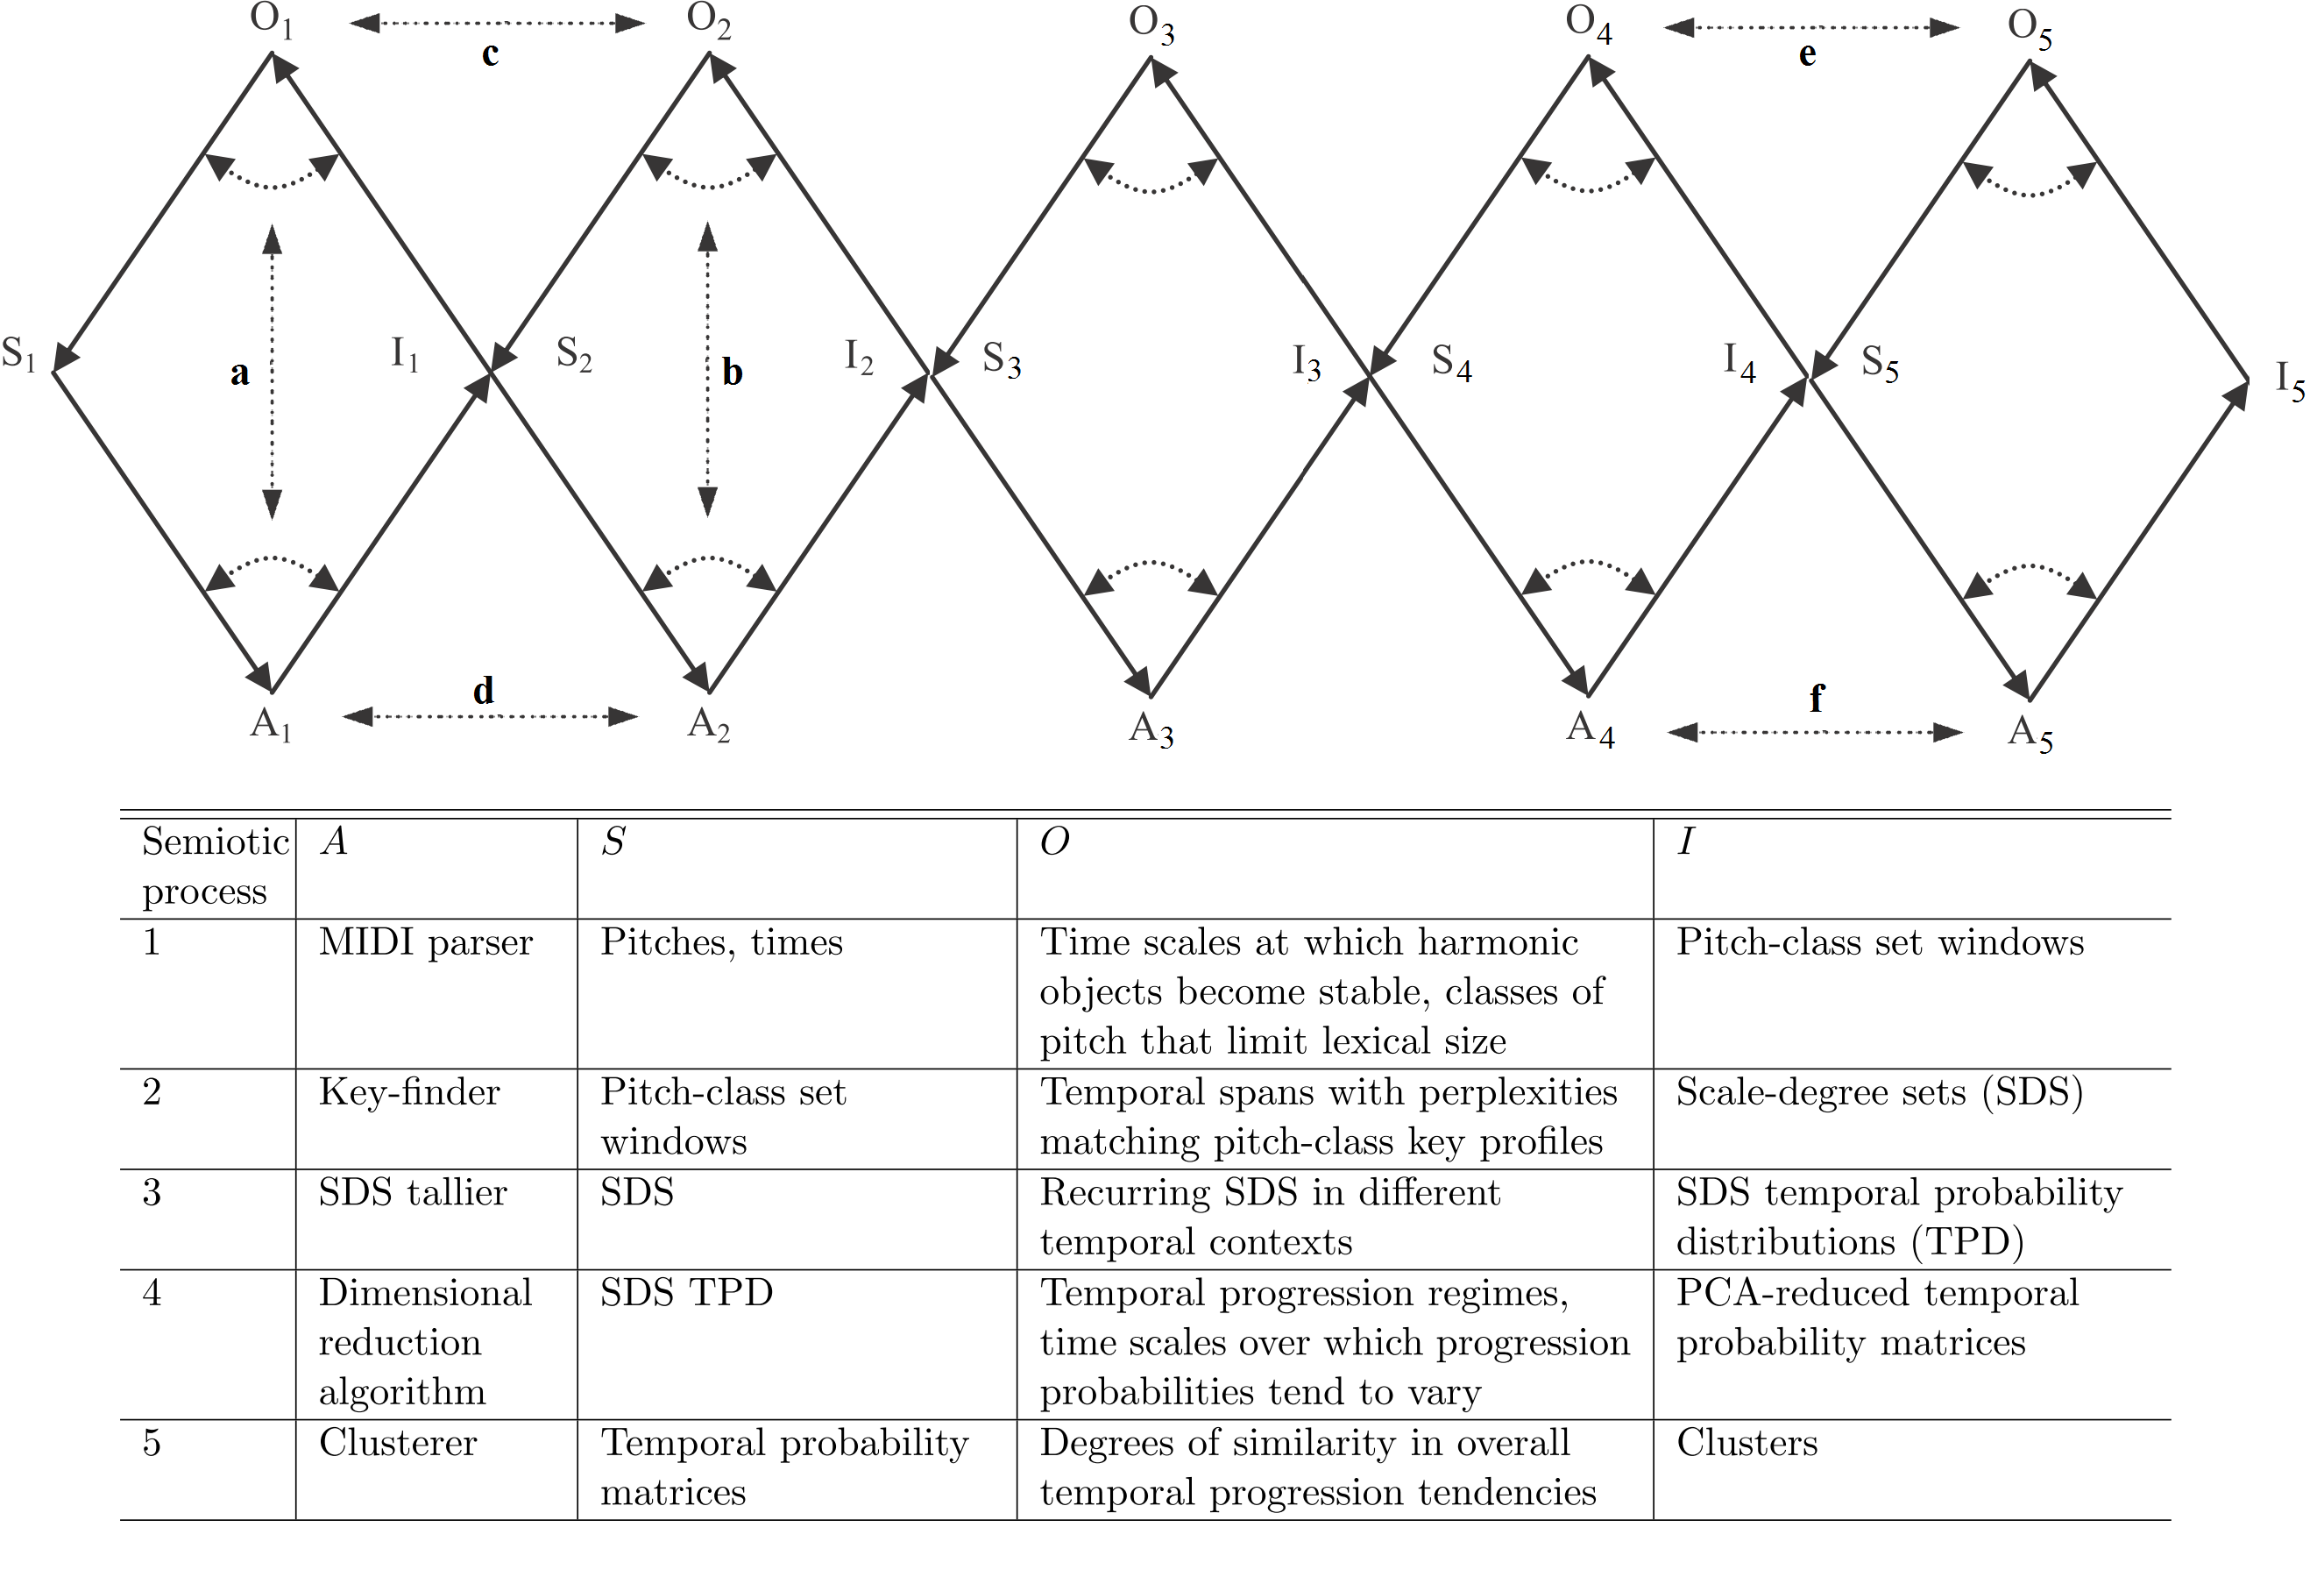
\includegraphics[width=8.25in]{kockelman_5jones.png}
\end{figure}
\end{landscape}


The objects $O_1$ occur at the smallest time scales where ``harmonies" -- roughly, collections with at least two or three pitches, as indicated by average window perplexity -- become stable, which tends to be around 50 milliseconds.  For $A_1$, time scales shorter than that sign some other kind of object or process, which a human might interpret as rolled chords with slightly different (but extremely close) onset times or very fast melodic runs.\footnote{Empiricists and interpreters alike tend to locate the shortest span for human auditory attention in this regime; see London 2012, who cites 100ms (p.\ 28) and Chion 2016 (p. 24), who cites 40ms.  That lends support to this choice of time scale, but the algorithm does not know this, and it did not choose it for this reason.}  $A_1$ does not know what these other objects are, of course, but it knows that the time scale at which it interprets objects $O_1$ is a special one -- special for the algorithm, in that it optimizes certain information-theoretic criteria, and special for us, in that it defines temporal objects well-suited to any theory purporting to treat chord progressions (e.g., the rest of the pipeline).

$A_1$ also assumes and generates objects with particular pitch properties.  For this agent, a voicing is not a chord; labeling each individual voicing type separately produces a very large and sparsely-populated vocabulary.  In order to select ``chords"  which may carry meaningful temporal progression statistics and recur across the corpus in many contexts (that is, to enable the task of the algorithmic agents with which it will communicate), $A_1$ turns pitch indices $S_1$ into pitch-class interpretants $I_1$.  This builds in a particular kind of ``bias," in Gjerdingen's sense (cf.\ Chapter 2), assuming that statements regarding harmonic progression might profit from this descriptive basis.  But \emph{any} analytical system involves labeling bias, and the relation between $A_1$ and the chord objects $O_1$ (given by dotted line (\textbf{a})) is chosen to align that bias with the specific conditions necessary for semiotic processes further down the pipeline.  If $A_2$ is coded and designed to use the interpretants produced by $A_1$ for a particular purpose (an inter-agent communicative relation indicated by arrow (\textbf{d})), then the properties ascribed to $O_1$ and $O_2$ ought to share modes of indexicality and significance (the (\textbf{c}) arrow).

%A_2: key-finder
After the MIDI parser ($A_1$) produces short-duration pitch-class set windows ($I_1$), the key-finder ($A_2$) interprets combinations of those windows as signs ($S_2$) indexing key spans ($O_2$).  As in relation (\textbf{a}), where the MIDI parser selects and interprets chord objects based on their distributional perplexity in time and a limited lexical size, the key-finder defines key spans as time windows with pitch-class perplexities similar to empirically-derived key profiles (Bellman-Budge, here, though other profiles have similar perplexities).  For $A_2$, spans governed by a particular key have no necessary chord structures, progressions, or cadential rhetoric -- they are defined by the relative proportion of scale degrees sounded during the span.\footnote{I note that assumptions regarding chord structure and progression may be read out of the key profiles, since scale degrees drawn from common roman-numeral chords receive high weightings, but the key-finder does not know this.}  Taken together, $A_1$ and $A_2$ trace a particular line of inquiry: if there is a time span at which harmonic objects first stabilize as quasi-verticalities, and if there is another time span at which the relative appearance of pitch-classes indexes or projects the distributional properties of key, then the scale-degree sets $I_2$ may be taken as consistently-defined labels for objects of harmonic interest.  $A_1$ and $A_2$ act as temporal filters, or as selecting ``sieves," in Kockelman's terms, each of which selects certain indices as significant toward the production of scale-degree set interpretants.

%A_3, sds-tallier
$A_3$, the scale-degree set tallier, has no direct access to the un-transposed MIDI data.  It examines the transposed scale-degree sets and time windows generated by the key-finder ($I_2 = S_3$), and it produces temporal probability distributions which make sense given progression objects (i.e., chords) specified by the ontology in which $O_3$ is embedded: each appearance of a particular scale-degree set indexes the general behavior of the scale-degree set across a token-type relation.  The tallier finds every token corresponding to a particular scale-degree set type (say, all performed instances of $[0,2,5,9]$) corpus-wide and records what other scale-degree set tokens appear within the subsequent five seconds (a span chosen based on the long-range predictivity of chords, which tapers off over time).  Each token has a particular temporal index (it is struck at exactly one time) and a specific sequence of other scale-degree set tokens which follow it.  The types, on the other hand, have a different ontological status: they do not occur at any particular time, and they are not associated with any specific sequence of chords.  Rather, the properties of each scale-degree set type consist of the probabilities with which many possible destination chords appear at given temporal delays.

This type-as-temporal-feature-bundle is a different kind of ``chord" object from $O_1$ or $O_2$, though its formation depends on them.  Crucially, the ontological difference between $O_2$ and $O_3$ is precisely the set of properties which permit generalizations regarding harmonic progressions.  When a jazz analyst claims that $V$ tends to go to $I$, he or she does not mean that a particular $V$ chord immediately proceeded to $I$ in one phrase of one performance.  The claim instead describes the frequent -- or most probable -- behavior of a type ``$V$" indexed by a wide variety of $V$ tokens.  The temporal probability distributions $I_3$ assigned to origin chord types $O_3$ encode that propositional relationship in explicit computational terms.  Unlike a human analyst, $I_3$ does \emph{not} say that a particular scale-degree set ``tends to go" anywhere, opting instead to provide a nuanced statistical portrait of what happens after each token appearance.  $I_3$ is not a judgment call; it is not a metaphysical claim; it makes no statement regarding what about a given scale-degree set might cause it to progress in any particular way; it does not even define exactly what a ``chord progression" might mean.  $I_3$ is a translation of facts communicated across and generated by the network of agents $A_1 \rightarrow A_2 \rightarrow A_3$.  It captures, in a minimal sense, the ontological shift necessary to move from statements regarding individual sonic moments $I_1$ or $I_2$ to generalizations about a chord type.  To my knowledge, every extant theory of harmonic syntax, function, or progression performs this ontological shift, but its nature is rarely specified -- indeed, for human-based analysis, it may be impossible to fully specify it.\footnote{Empirical or corpus analytical projects often perform this shift \emph{twice}, where individual tokens index types, and types generate or induce rules which then impact other tokens.  Human analysis which starts from categories constructed from notions of consonance or pitch content may only perform this shift \emph{once}, where the properties ascribed to a pre-defined category are inherited by tokens only during particular analysis.}  Here, the generalization receives statistical specification.

%A4: PCA reducer
If $A_3$ defines types from tokens, generalizing from many ``origin" chord instances to a far smaller number of indexed types, $A_4$ performs an analogous interpretation regarding chord-to-chord progressions in time.  For each origin chord scale-degree set, the dimensional reduction algorithm $A_4$ examines the probability distributions $I_3 = S_4$ which constitute the features ascribed to $O_3$.  How a chord (or rather chord \emph{type}) progresses is encoded in this data.  But statements regarding chord progression tendencies are not merely statistical portraits of nearby chords.  $A_4$ generalizes from the fine-grained temporal data to construct and define temporal progression regimes $O_4$ (cf.\ Chapter 3), ways of progressing in time.

%Human reduction
When a human analyst performs this reductive move, rhetoric, voice-leading, and phrase-level expectations inform distinctions between embellishing ``progressions," syntactic progressions, and chord-to-chord correlations deemed irrelevant to syntactic analysis.  Consider a temporally-ordered chord sequence $C_1, C_2, C_3,...,C_n$ for some large $n$.  Except under extraordinary circumstances, an analyst would rarely call the temporal correlation $C_1 \rightarrow C_{31}$ a ``progression."  But if $C_2$ and $C_3$ may be reduced away as voice exchanges or neighbor chords, the same analyst might well identify $C_1 \rightarrow C_4$ as a progression.  $A_4$ employs principal component analysis to produce similar types of ``progression" with a very different justification scheme.  Based on the temporal progression distributions, $A_4$ looks for combinations of time indices over which origin chord - destination chord combinations tend to show the highest variance in probability.  For most origin chords, a small number of components capture the lion's share of the variance in distributions, and the score given to each destination chord along each component indicates how well-captured its probabilistic variance is by that kind of temporal variance -- that mode of progression.\footnote{As indicated in Chapter 4, some caution is necessary here, as the (human) interpretation of a destination chord with high scores along more than one component is ripe for misinterpretation; does such a chord participate in more than one mode of ``progression," or do combinations of components themselves index modes of progression?}  $A_4$ may be thought to find chord progressions that a human would identify, but it really selects certain indices from the temporal probability distributions and assigns them as predicates for progression objects it constructs.

%A5: clusterer
Examining the temporal probability matrices in the dimensionally-reduced PCA basis ($I_4 = S_5$), the clustering algorithm ($A_5$) groups origin chords into categories of similar progression behavior $I_5$.  These clusters make sense in the presence of the temporal probability matrices $S_5$ only under the selection assumptions encoded in the clustering algorithm's optimization criteria and distance metric.  The properties of the chord cluster objects $O_5$ consist of the crude Manhattan distances between elements of each cluster.  Chords are ``similar" to one another if they are indexed by destination chords in statistically-similar ways across temporal progression regimes; since these properties depend on the indices selected by $A_4$, the relation between the dimensional reduction algorithm and the clusterer $A_4 \leftrightarrow A_5$ is mediated by the relation between the cluster objects and the temporal progression regimes $O_4 \leftrightarrow O_5$ (dotted arrows (\textbf{e}) and (\textbf{f}) on Figure~\ref{k_j}).

%incommensurability 
If one takes this semiotic chain as a black box $S_1 \rightarrow \blacksquare \rightarrow I_5$, where performances enter on one side and categories of chords come out the other, then the temptation to compare the black box to a brain and its outputs to human-generated categories of chord syntax is strong.\footnote{TODO: Think about whether and how much to unpack the computer science history of the black box, the Latourian implications of breaking it open like I do here.}  Indeed, the cognitive turn in corpus analytical music studies consists almost entirely of giving in to this temptation.  When David Temperley writes of a musical corpus that ``the model that makes the most accurate predictions about the data is then the most plausible model of the cognitive processes that gave rise to it," he assumes a fundamental similarity between algorithmic agents and processes in the human brain.\footnote{See Temperley 2010, p.\ 355.  Temperley could get out of this by defining ``model" in an ends-oriented way, but the degree to which the ``homunculus talk" is mitigated by that definition corresponds to the degree to which the ``model" could say nothing about cognitive processes.  (For a general critique of homunculus talk in cognitive research, see McGinn 2013 and the flurry of angry responses it generated from neuroscientists in the \emph{New York Review of Books}.)}  If a model clusters chords, for example, and produces results that mimic human-generated results, it may describe how humans make or perceive the music.  I intend the above framing to block this interpretation.  Not only do the algorithmic processes have no necessary neural correlates, but even the objects indicated -- the chords and categories and progressions selected, constructed, and interpreted by the algorithmic agents -- look like but \emph{are not} the objects of traditional (human) harmonic study.  That the clusters $I_5$ resemble traditional ideas regarding harmonic progression tendencies may be productive, useful, and applicable in a variety of circumstances (some of which I will elucidate below), but the semiotic referents upon which the algorithmic pipeline depends are fertile homophones, sounding like human statements but meaning something else.

\subsection{What do algorithmic agents know?  Or: Analysts as parasites.}
%All agents know stuff
As Wollheim notes of Loran, as Waters notes of Strunk, and as I note of Terefenko: what an analytical agent knows (or believes) informs the segmentation and classification processes on which that agent's activities and interpretants rely.  So what do the algorithmic agents of Figure~\ref{k_j} know?

$A_1$ knows the timescale at which collections of pitch classes tend to form, but not how they relate to one another; $A_2$ knows the timescale at which scale degrees tend to occur jointly in patterned ways, but not their ordering; $A_3$ knows the temporal ordering of token scale-degree sets, but not what general kinds and scales of ordering are important or common; $A_4$ knows that some particular temporal correlations underpin ordering patterns for any given origin chord, but not how origin chords relate to one another; $A_5$ knows how origin chord types relate to one another, but not any specific contexts.  Each agent acts as a sieve, filtering out indices to present as signed objects necessary for the next agent down the pipeline.

%the things we know are not fundamentally true
This prevents one kind of bias while enforcing another.  A certain form of hermeneutics is explicitly blocked, since particular expectations for chord type behavior cannot propagate backwards down the pipeline.  Where Loran's ostensibly-formal shape segmentation was informed by representational expectations further down the chain, no agent in the YJaMP pipeline has access to such information.  When $A_1$ segments a chord, it has no idea what the ultimate behavior of that chord might be or what any type it indexes could do.  But in each semiotic process given above, the kinds of properties the agent ascribes to each object have still been selected in a way suited to more than one task.  Put another way, many different ontologies might support the isolated selection processes of a given agent, and only some of those align with the processes employed by other agents.  There are many other ways to segment a musical surface into chords; $A_1$ chooses a particular way which provides exactly the indices necessary for $A_2$ (and so on).  I do not claim that this is the ``right" way -- emphatically the opposite.  I mean the above framing as a demonstration that there can be no ``right" way.

%parasitism
I embed temporal properties as far back into the pipeline as possible, but there is still no guarantee that the objects produced by the segmentation of $A_1$ and $A_2$ can produce or bear the kinds of properties required by agents $A_4$ and $A_5$.  Since each successive agent interprets the previous agent's interpretants in light of its own ontology, the signs necessarily afford (mis)direction toward other ends.  If this were not the case, $A_3$ could not produce temporal progression statistics from $A_2$'s scale-degree sets, since those sets all carried properties corresponding to distinct times and contexts.  Kockelman writes that if an object ``implies (embodies or indexes) other ends it might be directed to serve or indeed implies any way it may fail to serve an end (whether original or diverted)... [t]he parasite is whatever inhabits such implications."\footnote{Kockelman 2012, p.\ 15.}  I claim that any context-oriented interpretant of a kind similar to that produced by $A_3$, $A_4$, or $A_5$ is parasitic on any content-oriented labeling systems similar to those produced by $A_1$ and $A_2$.  ``Just as a sign may (be taken to) stand for the wrong object," Kockelman reminds us, ``a  sign may also give rise to the wrong interpretant.  In this way, to return to our parasites, the \emph{tokens} instantiated may fail to conform to the \emph{types} selected."\footnote{Kockelman 2012, p.\ 20.}  While membership in a given cluster, for example, is determined by type-level similarity in temporal progression statistics, membership in a given type $[0,2,5,9]$ is still assigned on the basis of the scale-degree content of a given token.  In the above pipeline, the contextual behavior of each token is embedded in the type's properties in a traceable way, but any resulting statements regarding the progression behavior of types is parasitic on chord tokens; content labels are misdirected to bear contextual properties.

%failure is inevitable
This is not a unique feature of the pipeline framed here.  In fact, this pipeline attempts to minimize the potential for parasitic misdirection, since the properties of literally every token are embedded in the properties of the scale-degree set types and clusters.  But once a probability distribution is calculated, information is lost about any given token.  The task of generalizing about harmonic progressions is inherently and unavoidably parasitic. So long as analysts (human or algorithmic) wish to produce interpretants identifying the temporal behavior of types indexed by pitch sets, pitch-class sets, scale-degree sets, or any other quasi-atemporal signs, the progressions we attribute to chord types will always misdirect token notation and permit failure.\footnote{If I want to sound really crazy, I could ask here if there can be such a thing as content-free labeling.  It seems like this might be possible with a radical re-orientation of harmonic inquiry, where each token is described purely in terms of its surroundings in some explicit way.  Would the results be tautological or impossible?}

\subsection{What can these interpretants do?}
%but failure is not always bad
This is not bad.  ``Failure," in a semiotic sense appropriate to the parasite, consists partly in cases where a token assigned to a type does not properly inherit or exhibit or index properties assigned to that type.  When in a particular phrase a chord does not behave as the chord's pitches might lead us to expect, analysis is not ruined.  By insisting (and demonstrating) that the many tokens with the same scale-degree content participate in a variety of progressions with statistically normative properties, we force open a door for hermeneutic interpretation and attentiveness to individuation.  A pipeline implicating no semiotic parasitism, it seems, would amount to a re-indexing of the input signs with no gains in generality.

A model which treats each individual token as its own type will not fail; an algorithm could reliably indicate which chord tokens succeed any temporally-specific token in the corpus at any time delay.  But such models do not reduce the complexity of the domain in any way, and some balance between failure and usefulness is required.  This balance (and the nature of the resulting semiotic failures and uses permitted) depends on the interpretive ends desired and pursued by the analyst at the end of the chain.  Several such analysts afforded by the pipeline of chapters 2-4, both algorithmic and human, appear below.

%new-paradigm affordances designed to take parasitic advantage of the pipeline
\begin{enumerate}
	\item If an analyst seeks a high-level portrait of general temporal behavior at phonetic, syntactic, or long-range time scales, he or she might employ another algorithmic agent to tally the cluster-to-cluster transitions occurring at that time scale.  There are many ways this might be done, but perhaps the simplest is to modify the scale-degree set tallier $A_3$ to view cluster tags as input signs $S_3^{\prime}$ and produce temporal probability distributions $I_4^{\prime}$ for where tokens from those clusters tend to progress.  The same PCA reduction techniques would apply to these new distributions, re-encoding temporal progression regimes on the set of clusters, rather than the lexicon of scale-degree sets.
	
For example, if we want to know where chords in cluster 8 ($[0,2,5,7,9],[0,2,5,9],[2,5,9]$) tend to progress, we need to make several decisions: we might count or rule out progressions which remain within the cluster (like $[2,5,9] \rightarrow [0,2,5,9]$), we might choose different time scales, and we might index those time scales with millisecond windows or PCA-reduced basis components.  Table~\ref{8_progs} consists of interpretants produced under one set of those conditions.  Here, the tallier excludes intra-category transitions and looks for the shortest-scale progressions that result, as indexed by large PCA component 1 scores.
	
	\begin{table}
	\centering
	\caption{The top PCA component 1 (short time scale) destination chord clusters for origin chord cluster 8.  If cluster 8 contains $ii$-like chords, we might note that nearly all of the prominent destination chord clusters are $V$-like.}
	\label{8_progs}
	\begin{tabular}{p{0.75in} | p{0.75in} | >{\raggedright}p{1in} | >{\raggedright\arraybackslash}p{1in} }
	\hline\hline
	Destination cluster & PCA1 loading & Cluster example & Human interpretant\\ \hline
	45 & 7.74 & $[2,5,7,9,10]$ & $v^9$\\ \hline
	9 & 7.22 & $[0,4,5,9]$ & $IV^7$\\ \hline
	14 & 5.36 & $[2,5,7,11]$ & $V^7$\\ \hline
	13 & 4.96 & $[5,7,9,11]$ & $V^9$\\ \hline
	23 & 4.53 & $[2,5,9,10]$ & $\flat VII^{M7}$?\\ \hline
	48 & 4.47 & $[5,7,11]$ & $V^7$\\ \hline
	59 & 2.82 & $[7,8,11]$ & ?\\ \hline
	\end{tabular}
	\end{table}
	
The table lists the destination chord cluster labels (column one) with highest PCA-1 scores (column two) in descending order.  These columns are the tallier's actual interpretants, while the remaining two columns are my attempt to re-attach humans to the output.  Column three lists a single scale-degree set I have selected from the destination cluster (the full contents of which are listed on Table~\ref{memb}), and column four provides my rough gloss of what that chord might resemble in traditional theory parlance.  The algorithmic agents here do not know that several of these clusters resemble one another (like the $V^7$ and $V^9$ chords) -- only that tokens from these clusters frequently appear at similar, short time scales after a token from cluster 8.  My roman-numeral interpretations are explicitly parasitic on the algorithmic interpretants.  The pipeline's statistics do not prove that, say, ``$ii$ chords go to $V^7$ chords," but they provide a statistical language for specifying a meaning for such statements in a way accountable to the performance data.  And as with the mysterious appearance of $\flat VII^{M7}$ in Table~\ref{8_progs}, cluster type-level progression claims often produce statements counter-intuitive to a human analyst.  (Does this stand in for subtonic-type cadences in place of the more expected dominant $\flat VII^7$?)  Statements of this kind regarding cluster type progression properties might lead a human analyst down a variety of productive lines of inquiry.  These type-level properties cannot readily accomplish token-level phrase-parsing tasks of the kind performed by Terefenko, Strunk, or Waters, but they may inform or generate the norms on which those parsings rely.
	
	\item  The pipeline's direct connection to certain performance indices affords the isolation of seemingly non-normative token behavior.  When tallying the progression behavior of $[2,7,11]$ as a type, two strange claims emerge from the pipeline: that $[2,7,11]$ belongs in cluster 12, which contains many unambiguous tonic scale-degree sets (cf.\ Table~\ref{memb}), and that it progresses on many occasions directly to $[0,5,9]$.  Were these seventh chords, blues progressions might readily contain them, but their triadic nature appears unstylistic when compared to similar statements made under traditional harmonic analysis paradigms.

Recalling that the type is parasitic on the token, we may employ a new algorithmic agent to search for specific times where this progression takes place in the corpus.  In this case, doing so allows us to identify that 80\% of the token occurrences of $[2,7,11] \rightarrow [0,5,9]$ appear in just two recorded tunes: Alex Dubovoy's performance of ``Stella by Starlight," and Joe McWilliams's performance of ``If I had You."  Both performances feature prominent intro and outro ``riffs," vamp-like progressions setting the stage for the sound-world of the tune.\footnote{TODO: Who writes about riffs and vamps?}  The $[2,7,11] \rightarrow [0,5,9]$ progressions appear almost exclusively in these intros/outros.  This might imply that different syntactic constraints operate in vamp-like, repetitive harmonic contexts, and that intros and outros lying outside the purview of a tune's head and chord progression might afford different kinds of progression from the rest of the tune.\footnote{TODO: Surely somebody writes about this.}  The progression is a ``special effect" of sorts, and the pipeline's failure to re-produce traditional expectation allows us to unearth this particular behavior.

It might also imply that vamp-like progressions defy the usefulness of the key-finding algorithm.  Figure~\ref{alex_outro} provides a MIDI readout in ``piano roll" format (keyboard pitch versus time) for Dubovoy's ``Stella" outro, which consists primarily of three major triads transposed in parallel -- $BM \rightarrow AM \rightarrow A\flat M$.  Here we see that the key-finding algorithm has interpreted $BM \rightarrow AM$ as $[2,7,11] \rightarrow [0,5,9]$ merely in an attempt to fit an unusual progression into a ``key."  The repeated vamp produces a very consistent pitch-class distribution over a span of tens of seconds which loosely matches a traditional key profile.  The strong presence of $\{B,D\sharp,F\sharp\}$, $\{A,C\sharp,E\}$, and $\{A\flat,C,E\flat\}=\{G\sharp,B\sharp,D\sharp\}$ produces roughly the key-weightings of the $EM$ profile, despite its rhetorical and cadential implausibility.  After Dubovoy finishes the last rotation of the head in $B\flat M$, he sidesteps the concluding tonic chord, replacing it with $BM$ and initiating the vamp.  Since the resulting progression does not resemble the $B\flat M$ material which preceded it, the keyfinder makes its best guess.  Note that the keyfinder \emph{is not wrong}, semiotically: the properties the algorithm applied to a ``key" are different from the properties a human might consider important.  Key assignment thus does not directly mimic human activity, but it still serves to isolate progressions for aggregate statistics -- the keyfinder assigns McWilliams's vamp a similarly-``wrong" key, which nevertheless allows the tallier to see a similarity in the two progressions.
	\begin{landscape}
	\begin{figure}
		\centering
		\caption{The final 25 seconds of Alex Dubovoy's performance of ``Stella by Starlight."  The vertical axis plots keyboard pitch, from low to high; the horizontal axis tracks time from left to right.  The red boxes indicate the consecutive major triads separated by a whole step that the scale-degree set producing keyfinder identifies as $[2,7,11]$ and $[0,5,9]$.}
		\label{alex_outro}
		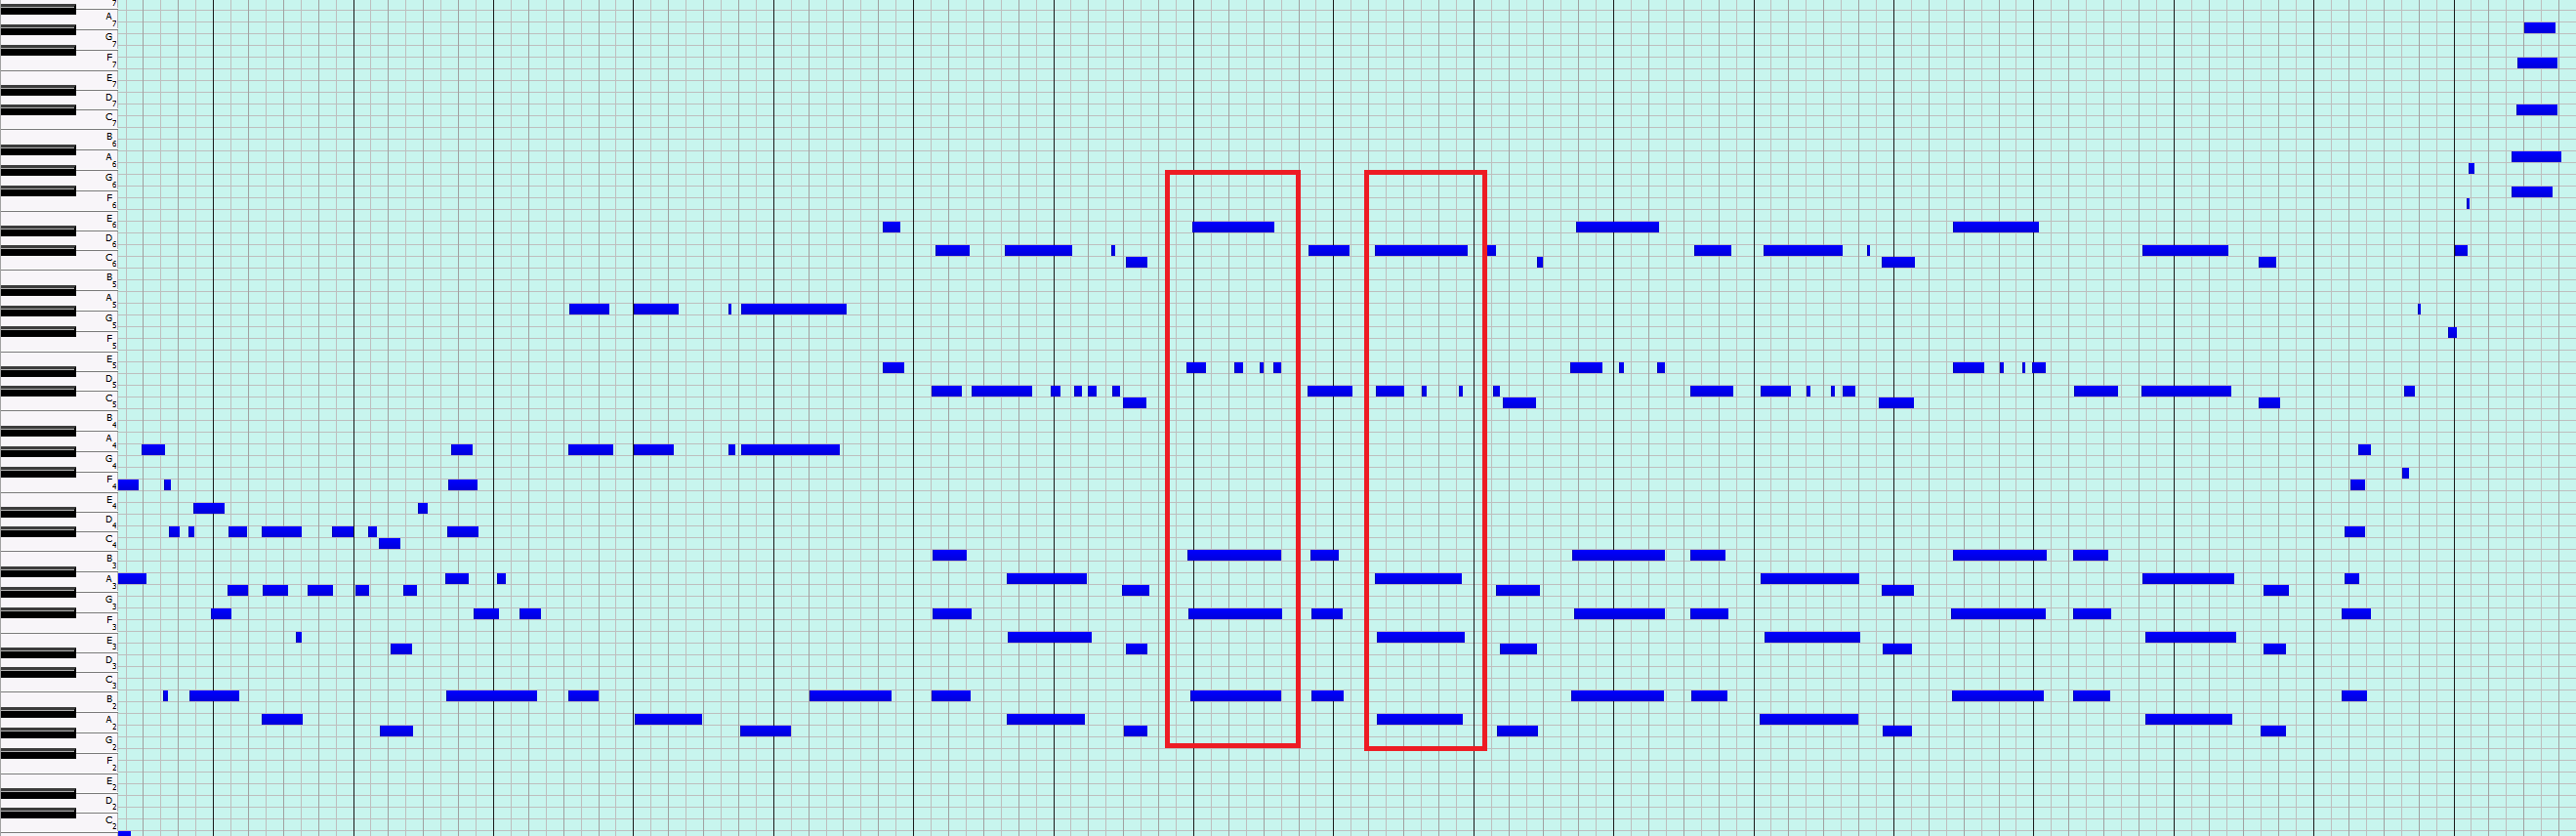
\includegraphics[width=8.75in]{alex_outro.png}
	\end{figure}
	\end{landscape}

Compared to a human analyst, the pipeline failed, both semiotically and practically -- this key parsing does not reflect human intuitions in a useful way.  But it (when combined with a human analyst) succeeded in locating a spot where normative key behavior is defied in an organized and systematic way.  To reproduce this mode of inquiry, a human analyst might compare his or her syntactic intuitions to progression-statistical interpretants produced by algorithmic agents and run the pipeline backwards, so to speak, to identify patterns captured by the type properties but about which we have no \emph{a priori} intuitions.  As I have argued elsewhere, corpus-analytical methods construct homogeneous harmonic norms while also providing a means for identifying and extracting their heterogeneous remainders.\footnote{I refer here to unpublished work I presented at the New England Conference of Music Theorists in 2015, ``Bach's `Gapped' Voicings, Expressive Meaning, and Part-Writing Pedagogy."}  Humans and algorithms disagree regarding what a key is, but this disagreement allows the YJaMP pipeline to sign patterned progressions outside frame reachable by other paradigms.

%Well-formedness rules, CCG grammars	
	\item Generally speaking, the behavior modeled by the cluster memberships and type progression probability distributions will prove more useful in aggregating normative corpus-wide trends than producing local parsings.  Linguistically-inclined analysts will note that the former kind of data guides the production of well-formedness rules like those employed at the end of the semiotic chain I attributed to Terefenko in Figure~\ref{k_t}.  To disambiguate potential parsings, Terefenko judges the possible functional category assignments ($I_2 = S_3$ on Figure~\ref{k_t}) by the degree to which they produce syntactically well-formed contextual phrases.  As my framing implies, such judgments rely on the properties of well-formed phrases or well-formedness rules ($O_3$).  Type-level cluster transition statistics provide one possible grounding for such rules drawn from a given corpus.
	
Sophisticated natural language processing (NLP) approaches to jazz analysis typically encode well-formedness rules into a grammatical model and assess their appropriateness based on how well they reproduce ``gold standard" analyses (usually produced by a human and from lead sheets).  Granroth-Wilding and Steedman 2012, for example, extends and employs earlier Combinatory Categorial Grammar (CCG) approaches to constrain lexical combinations based on the behavior of the categories to which they belong.  But as inputs for their grammatical parsings, the authors ``have hand-crafted a lexicon containing categories suitable for assigning harmonic interpretations to chords," and the resulting categories depend very strongly on their assumption that identifiable roots and chord qualities form the basis of syntactic categories.\footnote{Granroth-Wilding and Steedman 2012, p.\ 4.}  The pipeline of chapters 2-4 provides an alternate method for generating such a lexicon, and CCG or other grammatical methods might be employed to turn cluster assignments as signs into well-formed parsings as interpretants.

I leave open the question of what type of well-formedness rules would best capture the temporal progression behavior of YJaMP or any other jazz corpus, though (as Chapter 1 implies) I am skeptical of the deeply recursive hierarchical and semantic structure Granroth-Wilding and Steedman employ.  But the use of probabilistic grammars based on data-driven lexical categories and the production of temporal progression norms could allow an analyst to produce local parsing interpretants from the otherwise ill-suited type-level statistics given here.  Crucially, the lexical assignments offered here do not encode any pre-conceptions regarding harmonic norms other than that they involve locally-transposed near-verticalities and their relative deployments over time.%TODO: should I beef up my critique of what the goal of such modeling methods is?  Maybe I should check what part of that ought to go in chapter 1.  

%Algorithmic composition
	\item A set of well-formedness rules based on the norms of a corpus can do more than guide parsing choices.  From the earliest research on computational grammars in music studies, parsers have appeared alongside \emph{producers} of music, generative routines which leverage rules drawn from a corpus or encoded based on human intuitions in order to support algorithmic composition efforts.\footnote{See Fern\'{a}ndez and Vico 2013.}  The specific indices captured by the statistics drawn from YJaMP are well suited to such a task, as they already encode computational generalizations regarding temporal ordering at many time scales.  As a recent undergraduate computer science thesis at Yale demonstrated, comparatively simple stochastic grammars can take the temporal probability distributions producced here and use them to generate weighted distributions from which chords may be drawn at random.\footnote{See Zitomer (unpublished).}  The results do not produce jazz in a way that humans do, but they provide two distinct benefits: they open algorithmic composition to a much wider lexicon of chords than roman numeral or lead sheet chord symbol-based methods, providing a fertile extension to the lexical constraints of algorithmic composers like Kulitta.\footnote{Cite Donya.  Diss + what's the best paper?} And they encode temporal correlations at many time scales, allowing the development of sophisticated probabilistic models.

%Common to both grammatical parsings based on well-formedness rules and probabilistic composition approaches: Bayesian updating, especially in the context of Markov-type models.  This pipeline uniquely well-suited to temporally-sensitive Markov approaches, like the mixed-order models of Saul \& Pereira
	\item In general, both generating algorithmic compositions and constructing well-formedness rules applicable to individual phrase parsings involve choices regarding how to align permitted elements of the harmonic lexicon into syntactic temporal orderings.  The semiotic agents and interpretants of the YJaMP pipeline are uniquely well-suited to Markovian probabilistic models designed to produce and assess the likelihood of such orderings.  As with many corpus analytical approaches in music theory, consideration of this class of models involves engagement with research in computational linguistics.  In what remains, I will briefly frame a Markovian extension to the YJaMP pipeline suggestive for future work.
	
%explain classical n-gram Markov model, and shoot it down on temporal grounds
%footnote some n-gram models in music; bigrams and trigrams are good (like White?), but moving back farther than that is hard
Traditional $n$-gram modeling focuses on the moment at which a new or next chord's appearance in a sentence (linguistics) or progression (harmony) must be assessed probabilistically.  From a corpus of observation sequences, an $n$-gram model tallies all the ordered instances of $n$ consecutive tokens and produces probability distributions capturing what word (linguistics) or chord (harmony) tends to appear after every given combination of $n$ lexical elements.  Then, when the parser or generator encounters a sequence of elements $[C_1,C_2,C_3,...C_n]$ after which a new word or chord $C_{n+1}$ must be predicted, it draws on the knowledge encoded in the probability distributions -- after each sequence of $n$ elements, syntactically-structured corpora tend to display predictable patterns for the appearance of the $n+1$th element.\footnote{For a broader overview of $n$-gram methods, one can turn almost anywhere, these days -- but the textbook version given in Jurafsky and Martin 2000 is a lucid and thorough place to start.}

The choice of how much of a history to give each such moment hinges on the choice of $n$.  Considering a larger number of previous chords yields more finely-grained predictions, but the increased subtlety comes at the cost of extreme sparsity: for a lexicon of size $L$, a given $n$-gram distribution will need probability estimates for $L^n$ possible orderings.  Many of these orderings may never occur in the training set, and various ``smoothing" measures attempt to account for such events by re-allocating them low but non-zero probability.  Alternately, when $n$-gram models encounter a previously-unseen combination of $n$ elements, they may ``back off" to smaller orders $n-j$ in a variety of ways.  With such smoothing and backoff adjustments, $n$-gram models have proven highly adept at predicting word and chord sequences, despite their radical dependence on only the most local, ordered context.

White and Quinn, Rohrmeier and Cross, and Raphael and Stoddard, \emph{inter alia}, have implemented bigram and trigram models of harmonic progression ($n=\{2,3\}$) with demonstrable success from corpora represented as sequences of roman numerals or scale degree sets.\footnote{White 2013; Quinn and White?? ; Rohrmeier and Cross 2008; Raphael and Stoddard 2004.  Also cite HMM models like Mavromatis 2009, Bello and Pickens 2005 (MIR?).}  Rohrmeier and Cross's methods, in particular, stand as a relatively close analog to the YJaMP pipeline in this context, as they employ agglomerative clustering based on bigram transition statistics.  Their model, like other common $n$-gram implementations in music theory, avoids the large-$n$ sparsity problem by tallying only immediate chord adjacencies.

%transition to mixed-order Markov models
Like an $n$-gram model, the YJaMP temporal probability distributions inform the selection or likelihood of a new or next chord from the perspective of many temporally-previous chords.  But unlike common musical $n$-gram applications, a generative algorithm employing temporal data drawn from this pipeline may combine probabilistic contributions from each of the preceding chords individually at the time delay in question. Such an implementation would follow and extend the \emph{mixed-order} Markov model advocated in the linguistic context by Saul and Pereira.\footnote{See Saul 
\& Pereira 1997.}

%summarize Saul \& Pereira
Mixed-order Markov models, sometimes called ``skip-$k$" models, treat non-adjacent predictive correlations.  If considering $n>2$ consecutive words yields a sparse distribution, a standard back-off procedure might consider some smaller $n$. But the one or two closest words to a given token may be relatively uninformative for structured contexts with long-range dependencies.  Mixed-order models allow probability contributions from further back in the chain at placement delays; if the $n=3$ distribution for a given lexicon is sparse, for example, a mixed-order model might nevertheless make its prediction by considering only the word preceding the moment of prediction by three (or $k$) words (hence: skip-$k$).  As Saul and Pereira note, mixed-order Markov models incorporate more temporal information while retaining limits on the size of the distribution's lexicon, decreasing model perplexity without an explosion of sparsely-populated $n$-gram states.\footnote{See Saul 
\& Pereira 1997, Section 3.}

%Indicate analogous YJaMP pipeline interpretants
An algorithmic composer or parsing model could make analogous use of interpretants produced by the semiotic agents of the YJaMP pipeline.  For a given sequence of $n$ chords $[C_1,C_2,C_3,...C_n]$, an algorithm could assess the impact of each chord on the probable appearance of the $n+1$th chord with temporal probability distributions.  Since each $C_j$ for $1\leq j \leq n$ will fall at some temporal delay from $C_{n+1}$, its probabilistic contribution to the distribution from which $C_{n+1}$ will be drawn can arise from its distribution at time window $t= n+1-j$; this is precisely what is signed by the intepretants $I_3$ from Figure~\ref{k_j}.  Moreover, since each high-probability YJaMP origin chord can be associated with a PCA basis for its temporal progressions (by the dimensional reduction algorithmic agent $A_4$), a mixed-order algorithm could also take into account the time scales at which each particular $C_j$ tends to be most predictive, measured by PCA variance or distributional perplexity at $t=n+1-j$.  Chords with flat probability distributions at such times (like stable tonic chords at long $t$) could contribute less to the prediction of $C_{n+1}$ than chords with strong temporal correlations (like dominant-type chords at short $t$).  The very fact that the YJaMP pipeline generates chord types with detailed temporal properties that are difficult for a human to interpret renders its interpretants well-suited to such modeling.
\end{enumerate}

%sign off
%also nod to the fuzzy category assignment of aggregate Markov models, possibly name-drop factored language models? 
Each combination of agents above will draw on different indices and produce different interpretants, and each resulting pipeline must ensure that communicative ``failures" and parasitic re-interpretations push the research forward rather than hold it back.  If the preceding chapters offer anything of lasting use to a community of communicating agents with widely varied goals, I hope that its data representational paradigm imbricates temporality and semiotics in the production of harmonic syntax claims in a way which is flexible, generalizable, and aware of its limits.